%%%%%%%%%%%%%%%%%%%%%%%%%%%%%%%%%%%%%%%%%%%%%%%%%%
%  JASA LaTeX Template File
%  To make articles using JASA.cls, Version 1.1
%  September 14, 2019
%%%%%%%%%%%%%%%%%%%%%%%%%%%%%%%%%%%%%%%%%%%%%%%%%%

%% Step 1:
%% Uncomment the style that you want to use:

%%%%%%% For Preprint
%% For manuscript, 12pt, one column style

\documentclass[preprint]{JASA}

%%%%% Preprint Options %%%%%
%% The track changes option allows you to mark changes
%% and will produce a list of changes, their line number
%% and page number at the end of the article.
%\documentclass[preprint,trackchanges]{JASA}


%% NumberedRefs is used for numbered bibliography and citations.
%% Default is Author-Year style.
%% \documentclass[preprint,NumberedRefs]{JASA}

%%%%%%% For Reprint
%% For appearance of finished article; 2 columns, 10 pt fonts

% \documentclass[reprint]{JASA}

%%%%% Reprint Options %%%%%

%% For testing to see if author has exceeded page length request, use 12pt option
%\documentclass[reprint,12pt]{JASA}


%% NumberedRefs is used for numbered bibliography and citations.
%% Default is Author-Year style.
% \documentclass[reprint,NumberedRefs]{JASA}

%% TurnOnLineNumbers
%% Make lines be numbered in reprint style:
% \documentclass[reprint,TurnOnLineNumbers]{JASA}

\usepackage{natbib}


% Pandoc syntax highlighting

% Pandoc citation processing



\begin{document}
%% the square bracket argument will send term to running head in
%% preprint, or running foot in reprint style.

\title[A subtitle goes on another line]{Modeling trajectories using
functional linear first-order differential equations}

% ie
%\title[JASA/Sample JASA Article]{Sample JASA Article}

%% repeat as needed

\author{Julia Wrobel}
% ie
%\affiliation{Department1,  University1, City, State ZipCode, Country}
\affiliation{Colorado School of Public Health}
%% for corresponding author
\email{julia.wrobel@cuanschutz.edu}
%% for additional information

\author{Jeff Goldsmith}
% ie
%\affiliation{Department1,  University1, City, State ZipCode, Country}
\affiliation{Columbia University Mailman School of Public Health}
%% for corresponding author

%% for additional information


% ie
% \author{Author Four}
% \email{author.four@university.edu}
% \thanks{Also at Another University, City, State ZipCode, Country.}

%% For preprint only,
%  optional, if you want want this message to appear in upper left corner of title page
\preprint{Wrobel, JASA}

%ie
%\preprint{Author, JASA}

% optional, if desired:
%\date{\today}
\date{\today}

\begin{abstract}
% Put your abstract here. Abstracts are limited to 200 words for
% regular articles and 100 words for Letters to the Editor. Please no
% personal pronouns, also please do not use the words ``new'' and/or
% ``novel'' in the abstract. An article usually includes an abstract, a
% concise summary of the work covered at length in the main body of the
% article.
Put your abstract here. Abstracts are limited to 200 words for regular
articles and 100 words for Letters to the Editor. Please no personal
pronouns, also please do not use the words
\texttt{new\textquotesingle{}\textquotesingle{}\ and/or}novel'\,' in the
abstract. An article usually includes an abstract, a concise summary of
the work covered at length in the main body of the article.
\end{abstract}

%% pacs numbers not used

\maketitle

%  End of title page for Preprint option --------------------------------- %

%% See preprint.tex/.pdf or reprint.tex/.pdf for many examples


%  Body of the article
\hypertarget{introduction}{%
\section{Introduction}\label{introduction}}

\label{sec:intro}

Our motivating data comes from a study that collected 3D trajectories of
paw position over time as a mouse made a trained reaching motion for a
food pellet; the paw reach trajectories were measured concurrently with
neural activity in the motor cortex, an area of the brain known to be
important for voluntary movement. These data were collected in an effort
to understand the relationship between neural activity and paw movement.
This is an example from the increasingly common class of problems where
outcome and responses are measured densely in parallel. For these data
streams, we want to understand the relationship between inputs and
outputs that are both functions measured on the same domain. Recent work
using these data suggests that the dynamics of the arm during dexterous,
voluntary movements are tightly coupled to neural control signals from
the motor cortex \citep{guo2015, sauerbrei2018}.

To better quantify how brain activity affects current and future paw
position, we need a method that (1) allows future position to depend on
past but not future neural firing rate, (2) allows future position to be
affected by initial position, (3) has parameters that model the
relationship between the paw trajectory and the brain as a dynamical
system of inputs and outputs, the state of which evolves over time, and
(4) can accommodate repeated functional observations across trials.
These problems cannot be simultaneously addressed by current methods. We
develop a novel regression framework that combines ordinary differential
equations (ODEs) and functional regression and is well-suited to address
the problems our data presents. This work is connected to both the ODE
and functional data analysis literatures, which we review in Sections
\ref{sec:odes} and \ref{sec:fda}, respectively. First, in Sections
\ref{sec:data} and \ref{sec:flode}, we describe our motivating data and
model structure in more detail.

\hypertarget{paw-trajectory-data}{%
\subsection{Paw trajectory data}\label{paw-trajectory-data}}

\label{sec:data}

The motivating data were collected as part of a study on the specific
role of the motor cortex in enacting skilled movement, where a skilled
movement is defined as a voluntary behavior that requires coordination
and precision. Several experiments from \cite{guo2015} and
\cite{sauerbrei2018} show that the motor cortex generates a continuous
signal driving reach-to-grasp movements in mice.

In the experimental framework that generated our motivating data, a
single mouse was trained to reach for a food pellet in a memorized
location after hearing an auditory cue. The mouse was fixed at the head
to reduce variability in posture, the auditory cue was played, and the
mouse enacted the task of picking up its paw from a resting location to
reach for and grasp the food pellet. Video recordings of the task
completion were used to extract 3D trajectories of paw position from
lift (the point at which the paw leaves its rest position) to grasp (the
point at which the paw grasps the food pellet). An electrode array was
inserted into motor cortex to simultaneously record the spike times of
25 neurons. This describes a single trial of the experiment, which was
repeated 147 times.

For each trial \(i\), paw position was recorded in the \(x\), \(y\), and
\(z\) directions over 4 seconds, resulting in trivariate functional
observations \(\{ Y_i^{P_x}(t), Y_i^{P_y}(t), Y_i^{P_z}(t)\}\). Because
we treat each direction independently, going forward we simplify
notation to \(Y_i(t)\) by omitting the superscripts \(P_x\), \(P_y\),
and \(P_z\). The auditory cue was played 0.5 seconds into the trial, on
average lift occurred at 0.77 seconds, and on average grasp occurred at
0.88 seconds into the trial. For our analysis we limit the time frame to
the period 0.05 seconds before lift to 0.25 seconds after lift for each
trial, and data is linearly shifted so that the timing of lift for each
trial is aligned.

\begin{figure}
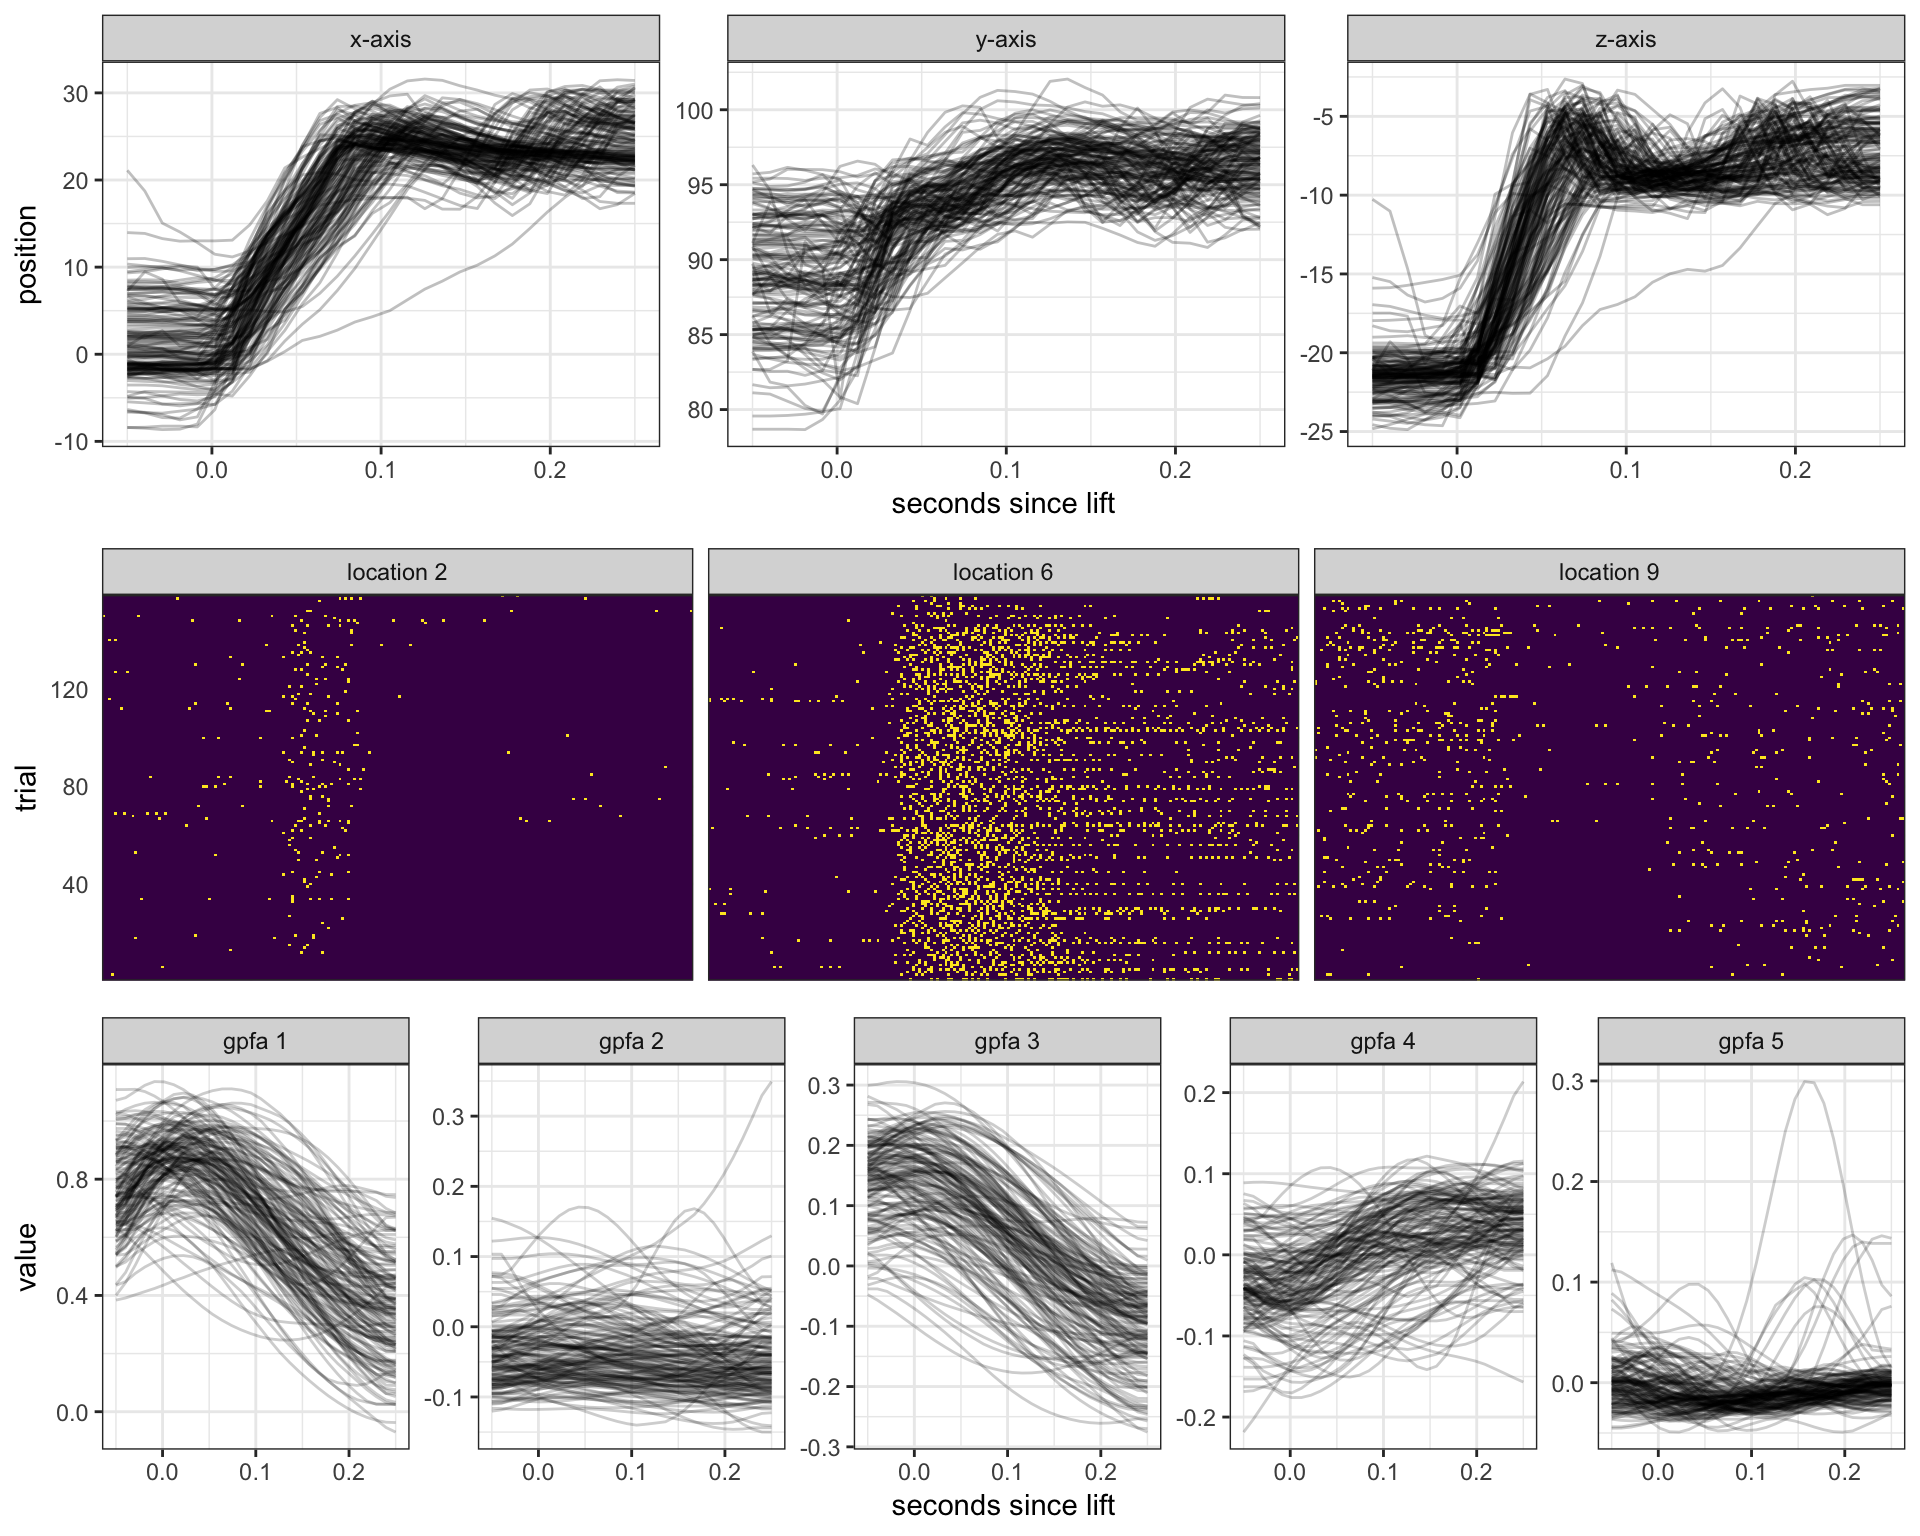
\includegraphics[width=\reprintcolumnwidth]{figs/fig_data_eda-1} \caption{Top row: Paw trajectories along $x$, $y$, and $z$ axes for 147 trials. Middle row: neural firing rates for 3 of the 25 neurons. Each row is a trial and each column is a point in time, and dark or light shading indicates that a neuron is off or on, respectively, at that point in time. After auditory cue, neurons show light activation at location 2, high activation at location 6, and dampening in activation at location 9. Bottom row: The five factors from Gaussian process factor analysis, shown for all 147 trials.}\label{fig:flode_data}
\end{figure}

The top row of Figure (\ref{fig:flode_data}) shows the paw positions
across trials and axes, from 0.05 seconds before lift to 0.25 seconds
after lift. Across axes, paw position at time \(t\) depends on initial
paw position at the start of the trial. The middle row of Figure
(\ref{fig:flode_data}) shows heat maps of the first 2 seconds of neural
activity for 3 of the 25 neurons, which were chosen because they are
representative of patterns seen across neurons. In figures showing
neural spike times, each row is a trial and each column is a point in
time; dark or light shading indicates that a neuron is off or on,
respectively. After the auditory cue at 0.5 seconds, neurons at location
2 are mildly activated, neurons at location 6 are highly activated, and
neurons at location 9 become less activated. Activity within neurons was
fairly consistent across trials, but large differences are seen across
neurons.

Firing rates of the 25 neurons were reduced to five dimensions using
Gaussian process factor analysis (GPFA), a standard technique for
decomposing noisy neural spiking activity into smooth low-dimension
neural trajectories \citep{yu2009}. From a neurobiological perspective,
extracting emergent patterns in the motor cortex using GPFA is a better
way of assessing how neural activity drives behavior than using the raw
neural firing data, because it increases generalizability across neurons
and trials. From a statistical perspective, GPFA also reduces risk of
collinearity when using the neural firing rates as covariates in a
regression setting.

Previous work used initial position and neural activity data to predict
paw trajectories for held-out trials. However, this work did not allow
for the relationship between position and neural activity to vary over
time, and did not enhance interpretation of this system of inputs and
outputs. We describe our model below; this work introduces a novel
regression method that is well-suited to our scientific context.

\hypertarget{flode-model}{%
\subsection{flode model}\label{flode-model}}

\label{sec:flode}

The biological underpinnings of our data are a dynamical system where
initial position and paw are being acted on by outside forces coming
from the motor cortex; these forces drive changes in velocity of the paw
which then influences position. We introduce the \emph{flode}
(\textbf{f}unctional \textbf{l}inear \textbf{o}rdinary
\textbf{d}ifferential \textbf{e}quation) model, a novel functional
regression framework that represents this neurobiological system of
inputs (motor cortical activity) and outputs (paw position). The
\emph{flode} model is a first-order ordinary differential equation
(ODE), which allows us to incorporate how change in paw position
influences position at time \(t\), reflecting the dynamic nature of our
data. In its differential form, our model is

\begin{equation}
\label{eq:flode_deriv}
y'_i(t) = -\alpha y_i(t) + \delta_i(t) + \mathcal{B}_0(t) + \sum_{p = 1}^P \mathcal{B}_p(t) x_{ip}(t),
\end{equation}

\noindent where \(y_i(t)\) and \(y'_i(t)\) are the paw position and
first derivative of paw position (velocity) at time \(t\),
\(x_{ip}(t), p \in 1\ldots P\) are trial-specific forcing functions, and
\(\alpha\), \(\delta_i(t)\), and \(\mathcal{B}_p(t), p\in 0\ldots P\)
are parameters to be estimated from the data. Forcing functions,
analogous to covariates in a traditional regression model, are external
input forces that act on the ODE system.

This is a buffered system, meaning the response time is longer than the
time interval in which the input changes. The scalar parameter
\(\alpha\), called the buffering parameter, indicates the amount of
buffering on the system. As \(\alpha \to 0\), buffering increases, and
the effects of forcing functions and initial position persist in time.
As \(\alpha\) grows larger, the effects of forcing functions and initial
position becomes instantaneous. The \(\mathcal{B}_p(t)\) are coefficient
functions that measure the impact of changes in the forcing function
\(x_{ip}(t)\) on the system, interpreted as the change in paw velocity
at time \(t\), \(y'_i(t)\), given a one unit change in forcing function
\(x_{ip}(t)\). \(\mathcal{B}_0(t)\) and \(\delta_i(t)\) are the
population-level and trial-specific intercepts, respectively. The
\(\delta_i(t)\) terms capture residual within-trial correlation; while
much of fine motor control is known to be driven by the motor cortex,
other brain regions also contribute to the paw reaching motion, and the
\(\delta_i(t)\) term is intended to capture changes in position driven
by unmeasured influences.

Many systems of differential equations cannot be solved analytically,
which makes traditional statistical estimation techniques with the
observed data \(Y\) as the outcome challenging. However, the class of
ODEs we consider has a solution, which we parameterize in terms of the
initial value, given by

\begin{equation}
\label{eq:flode_mod}    
    Y_i(t) = y_i(0)e^{-\alpha t} + \int_0^t e^{-\alpha (t-s)}\delta_i(s)ds + \sum_{p=0}^P\int_0^t e^{-\alpha (t-s)} \mathcal{B}_p(s)x_{ip}(s)ds + \epsilon_i(t).
\end{equation}

\noindent We make a distinction between \(y_i(t)\), the true
(unobserved) paw position at time \(t\), and \(Y_i(t)\), the paw
position at time \(t\) observed with measurement error
\(\epsilon_i(t)\). Thus, in model (\ref{eq:flode_mod}) above, we assume
the outcome \(Y_i(t)\) is measured with error but depends on the true
initial position \(y_i(0)\).

The \emph{flode} model is a first-order linear differential equation,
which reflects the biological process that is hypothesized to generate
the observed data. To familiarize readers with ordinary differential
equations and their use in statistics, we review the ODE literature in
Section \ref{sec:odes}. An overview of the functional data analysis
literature dedicated to regression, provided in Section \ref{sec:fda},
is also pertinent since the paw trajectories will be conceptualized and
modeled as i.i.d. realizations of functions that are observed over time.

\hypertarget{odes}{%
\subsection{ODEs}\label{odes}}

\label{sec:odes}

Systems of ordinary differential equations (ODEs) can be used to
directly model the relationship between an outcome and its derivatives,
leading to widespread popularity for modeling dynamical systems in
physics, biology, neuroscience, and other disciplines. First-order ODEs,
which incorporate only the first derivative of \(y\), follow the form
given in Equation (\ref{eq:flode_deriv}), though the \(\delta_i(t)\)
term we include is unconventional.

Equation (\ref{eq:flode_deriv}) is also said to be a linear differential
equation because its right hand side can be written as a linear
combination of \(y\) and terms that do not contain \(y\)
\citep{tennenbaum1985}. Though more complex ODEs are possible, such as
those of higher order or with nonlinearity, we believe the simpler model
can capture the dynamics of our data. When analytically solvable, most
ODEs do not have a unique solution. It is therefore common, and useful
for our data setting, to solve in terms of the initial value \(y(0)\).

Most applications of ODEs in science and engineering focus on
restrictive rather than general settings, in part because parameter
estimation for general models is challenging. In the past this
specificity has limited their use in statistics, but they are growing in
popularity. \cite{chen2017} reconstructs gene regulatory networks by
estimating sparse nonlinear ODEs for noisy gene expression data,
building on previous work \citep{lu2011, henderson2014}.

In their instant classic Dynamic Data Analysis, \cite{ramsay2017}
conceptualize dynamical systems as data-driven statistical models. The
book provides a framework for estimating a large class of differential
equations, as well as an excellent overview of ODE-based models that
expands on earlier work from \cite{ramsay2007} for parameter estimation
in nonlinear ODEs. Separate estimation frameworks are provided for
linear and nonlinear ODEs though both involve a tradeoff between the
best fit to a particular prespecified ODE and a smooth fit to the data,
enforced using B-spline expansions. While this general framework is
well-suited to estimate parameters for a single realization of an ODE,
it does not accommodate multiple trials or the complexities that arise
in that case.

\hypertarget{functional-regression-models}{%
\subsection{Functional regression
models}\label{functional-regression-models}}

\label{sec:fda}

Our data setting and proposed methods are also closely related to
functional data analysis. In functional data analysis, curve \(Y_i(t)\)
is the fundamental unit of statistical analysis \citep{ramsay2005}, and
functional analogs of univariate methods like regression, PCA, and
others build on this framework. Functional regression models capture the
relationship between outcome curves \(Y_i(t), i \in 1 \ldots N\) from
\(N\) independent trials, and the covariate(s) \(x_i\), which can be
scalar or functional. In particular, function-on-function regression
allows for both functional responses and functional predictors that can
be observed on different domains, and the response is related to the
predictor through integration of a coefficient surface
\citep{ramsay2005}.

Some special cases of function-on-function regression include the linear
functional concurrent model \citep{fan2008, goldsmith2017} and the
historical functional regression model \citep{malfait2003}. The
concurrent model uses the current value of the predictor to measure the
response at each time, but doesn't allow the covariates to affect future
values of the response. The historical functional model allows the
response at time \(t\) to be influenced only by the predictors up to
time \(t\); this is ideal for data where the response and predictor are
measured on the same domain, and prevents future values of the
predictors from influencing the present value of the response. Advances
in functional regression and accompanying software allow for historical
functional regression models with scalar and functional covariates, as
well as functional trial-specific random effects
\citep{scheipl2015, scheipl2016, refund}. The historical model with
trial-specific random intercept \(\gamma_i(t)\) is given by

\begin{equation}
\label{eq:fhist_mod}    
Y_i(t) = \gamma_i(t) + \beta_0(t) +  \sum_{p = 1}^P \int_{s = 0}^t \beta_p(t,s) x_{ip}(s)ds+ \epsilon_i(t).
\end{equation}

\noindent Here \(\beta_0(t)\) is the population-level intercept, and
each \(\beta_p(t,s)\) is a coefficient surface. This flexible model is
designed to handle repeated functional observations, and inclusion of
the random intercept \(\gamma_i(t)\) accounts for within-trial residual
correlation in the errors after modeling the relationship between the
outcome and the covariates curves.

Conceptually both the integrated \emph{flode} model in
\ref{eq:flode_mod} and historical functional regression use predictors,
including their recent history, to understand current values of the
response function. Because of these high-level similarities we find it
useful to compare and contrast these methods. If we assume the surface
\(\beta(t,s)\) from Equation (\ref{eq:fhist_mod}) takes the form
\(e^{-\alpha (t-s)} \mathcal{B}(s)\) from Equation (\ref{eq:flode_mod}),
\(\gamma_i(t) = y_i(0)e^{-\alpha t} + \int_0^t e^{-\alpha (t-s)}\delta_i(s)ds\),
and \(\beta_0(t) = \int_0^t e^{-\alpha (t-s)}\mathcal{B}_0(s)ds\), then
\emph{flode} can be considered a special case of the historical
functional regression model. However, the \emph{flode} surface
\(e^{-\alpha (t-s)} \mathcal{B}(s)\) is very restricted compared to the
more general historical surface \(\beta(s,t)\); as a result, the
historical model is likely too flexible and may overfit data that is
generated by the \emph{flode} model.

These assumptions are not trivial. From a conceptual standpoint,
\emph{flode} introduces a new framework for thinking about the
relationship between inputs and outputs in an ODE system, and the
historical model does not offer this interpretation. Initial position is
a crucial element of the \emph{flode} framework because it provides a
specific analytic solutions to the ODE in \ref{eq:flode_deriv}; in
contrast initial position is not a natural element of the historical
model and does not have precedent in the functional regression
literature. Explicitly incorporating initial position into a functional
regression context is both critical for our dynamical systems approach
and a novel contribution in its own right. Finally, the \emph{flode}
model is nonlinear in its parameter \(\alpha\), a development which
other functional regression methods haven't directly addressed.

\hypertarget{methods}{%
\section{Methods}\label{methods}}

\label{sec:methods}

Our work introduces models (\ref{eq:flode_deriv}) and
(\ref{eq:flode_mod}), a novel framework for modeling functional
observations with an explicit dynamical systems interpretation.

\hypertarget{model-formulation}{%
\subsection{Model formulation}\label{model-formulation}}

The \emph{flode} method is a system of differential equations, where
equation (\ref{eq:flode_deriv}) represents the model on the scale of the
paw velocity, and equation (\ref{eq:flode_mod}) on the scale of the paw
position. Because we observe paw position data rather than paw
velocities, we estimate parameters using the paw position model.
However, we are interested in interpretation on the velocity scale.

In this section we explain our parameter estimation approach. The
buffering parameter \(\alpha\) will be estimated using nonlinear least
squares. Since we observe initial position with error, \(Y_i(0)\), we
also need to estimate true initial position, \(y_i(0)\). The random
effects \(\delta_i(t)\) and coefficient functions \(\mathcal{B}_p(t)\)
will be estimated using penalized splines. Under these conditions all
parameters will be estimated jointly using the algorithm described in
Section \ref{sec:em_algorithm}.

To induce smoothness and reduce dimensionality, the trial-specific
random intercepts \(\delta_i(t)\) and coefficient functions
\(\mathcal{B}_p(t)\) are expanded using a fixed B-spline basis,
\(\mathbf{\Theta}(t)\), of \(K_t\) basis functions
\(\theta_1(t),\ldots , \theta_{K_t}(t)\), such that
\(\delta_i(t) = \mathbf{\Theta}(t)\mathbf{d}_i\) and
\(\mathcal{B}_p(t) = \mathbf{\Theta}(t)\mathbf{b}_p\), where
\(\mathbf{d}_i\), \(i \in 1\ldots N\) is a \(K_t \times 1\) vectors of
spline coefficients for the random intercept of the \(i\)th trial, and
\(\mathbf{b}_p\), \(p \in 0, \ldots, P\) is a \(K_t \times 1\) vector of
spline coefficients for the \(p\)th coefficient function. Using this
representation each forcing function term becomes

\begin{eqnarray*}
\sum_{p=0}^P \int_{s=0}^t e^{-\alpha (t-s)} \cdot x_{ip}(\mathbf{s}) \cdot \mathcal{B}_p(s) ds &=&\sum_{p=0}^P \int_{s=0}^t e^{-\alpha (t-s)} \cdot x_{ip}(s) \cdot  \Theta(s)\mathbf{b}_p ds \\[5mm]
&=& \sum_p \left(\int_{s=0}^t \left[\{e^{-\alpha (t-s)}\cdot x_{ip}(s)\}\otimes 1^T_{K_t}\right] \cdot \Theta(s) ds\right)\mathbf{b}_p \\[5mm]
&=& \sum_px_{ip}^*(t, \alpha)\mathbf{b}_p\\
&=& \mathbf{x}_i^*(t, \alpha)\mathbf{b},
\end{eqnarray*}

\noindent where \(\otimes\) denotes the element-wise Kronecker product,
and \(1_{K_t}\) is a length \(K_t\) column vector with each entry equal
to 1. We define a \(D \times \{K_t \times (P + 1)\}\) matrix
\(\mathbf{x}_i^*(t, \alpha) = \left\{x_{i0}^*(t, \alpha) | \ldots | x_{iP}^*(t, \alpha) \right\}\)
and a \(\{K_t \times (P + 1)\} \times 1\) vector
\(\mathbf{b} = \left(\mathbf{b}_0^T | \ldots | \mathbf{b}_P^T \right)^T.\)
Similarly, the random intercept term becomes

\begin{eqnarray*}
 \int_{s=0}^t e^{-\alpha (t-s)} \cdot \delta_i(s)ds &=&   \int_{s = 0}^t e^{-\alpha (t-s)} \cdot \Theta(s)\mathbf{d}_i ds\\[5mm]
&=&  \left[\int_{s = 0}^t \left\{ e^{-\alpha (t-s)}\otimes 1^T_{K_t} \right \}\cdot \Theta(s) ds\right] \mathbf{d}_i  \\[5mm]
&=& \mathcal{D}^*(t, \alpha)\mathbf{d}_i,
\end{eqnarray*}

\noindent Finally, we define
\(y_{i0}^*(t, \alpha) = y_i(0)e^{-\alpha t}\).

Though the conceptual model is expressed over continuous time domain
\(t\), in practice, each trajectory \(Y_i\) is observed on the discrete
grid, \(\mathbf{t} = \{t_1, t_2, \ldots, t_D\}\), which we assume to be
equally spaced and shared across trials. Functions \(Y_i(\mathbf{t})\)
evaluated on this grid are vectors of length \(D\), and
\(\mathcal{D}^*(\mathbf{t}, \alpha)\) and
\(x_{ip}^*(\mathbf{t}, \alpha)\) are \(D \times K_t\) matrices. Letting
\(\mathbf{\Theta}(\mathbf{t})\) be the \(D \times K_t\) spline matrix
evaluated at \(\mathbf{t}\), then
\(\delta_i(\mathbf{t}) = \mathbf{\Theta}(\mathbf{t})\mathbf{d}_i\) and
\(\mathcal{B}_p(\mathbf{t}) = \mathbf{\Theta}(\mathbf{t})\mathbf{b}_p\).
Putting these terms together and evaluating on grid \(\mathbf{t}\) gives
the observed data model,

\begin{equation}
\label{eq:observed_mod} 
    Y_i(\mathbf{t}) = y_{i0}^*(\mathbf{t}, \alpha) +  \mathcal{D}^*(\mathbf{t}, \alpha)\mathbf{d}_i +  \mathbf{x}_i^*(\mathbf{t}, \alpha)\mathbf{b} + \epsilon_i(\mathbf{t}).
\end{equation}

\noindent We use the notation \(g^*(t, \alpha)\) above to highlight that
terms \(\mathbf{x}_i^*(t, \alpha)\), \(\mathcal{D}^*(t, \alpha)\), and
\(y_{i0}^*(t, \alpha)\) are all functions of both time \(t\) and the
model parameter \(\alpha\). However, throughout this section these terms
will be used interchangeably with the terms \(\mathbf{x}_i^*\),
\(\mathcal{D}^*\), and \(y_{i0}^*\) for notational simplicity.
Naturally, on a discrete grid the integral defined above needs to be
approximated numerically. For numeric integration we use a Riemannian
approach, but other approaches would be reasonable as well.

We assume both the spline coefficients for the trial-specific intercept,
\(\mathbf{d}_i\), and the white noise, \(\epsilon_i(t)\), are random and
have the following distributions

\[\epsilon_i(t) \sim N(0, \sigma^2I_D)\]
\[\mathbf{d}_i \sim N(0, \Sigma_{Kt\times Kt}),\]

\noindent which induces a conditionally normal distribution on the
observed data given the random effects,

\[Y_i| \mathbf{d}_i \sim N\left(y_{i0}^* + \mathcal{D}^*\mathbf{d}_i+  \mathbf{x}_i^*\mathbf{b}, \sigma^2I_D \right).\]

\noindent Penalization is a popular technique to avoid overfitting in
functional models which we emply here for both random and fixed effect
spline coefficients. For fixed effect spline coefficients
\(\mathbf{b}_p; p\in 0,\ldots,P\), we assume
\(\mathbf{b}_p \sim N(0, \lambda_{b,p}\mathcal{P}^{-1})\), which
introduces a smooth penalty on the coefficient functions. Similarly, we
assume the random intercept variance is
\(\Sigma_{Kt\times Kt} = \lambda_d\mathcal{P}^{-1}\). Here
\(\mathcal{P}^{-1}\) is a known penalty matrix that is shared across
fixed and random effects to enforce a common penalty structure.

We estimate the buffering parameter \(\alpha\), variance parameters
\(\sigma^2\) and \(\lambda\), true initial positions \(y_i(0)\), and
spline coefficients \(\mathbf{b}\) and \(\mathbf{d}_i\) using the
expectation-maximization algorithm described in below. The algorithm
incorporates a nonlinear least squares step to optimize the \(\alpha\)
parameter.

\hypertarget{em-algorithm-for-estimating-fixed-and-random-effects}{%
\subsection{EM algorithm for estimating fixed and random
effects}\label{em-algorithm-for-estimating-fixed-and-random-effects}}

\label{sec:em_algorithm}

We use an expectation-maximization (EM) algorithm to find the maximum
likelihood estimates (MLEs) of both fixed and random effects, following
precedent from \cite{laird1982} for longitudinal data and
\cite{walker1996} for nonlinear mixed models. Our goal is to estimate
the experiment-wide fixed effects
\(\mathbf{\Phi} = \left\{\alpha, \mathbf{b}, y_i(0), \sigma^2, \lambda_d, \lambda_{b, 0}, \ldots, \lambda_{b, P}\right\}\)
and the random effect spline coefficients \(\mathbf{d}_i\). In the
\(M\)-step of the algorithm we estimate the MLE of the fixed effects
when the random effects are observed,
\(\widehat{\mathbf{\Phi}} = \underset{\mathbf{\Phi}}{\mathrm{argmax}}\{l(\mathbf{\Phi} | Y)\}\),
and in the \(E\)-step we get estimates for the random effects by taking
the expectation of the \(\mathbf{d}_i\) under the posterior distribution
of \(\mathbf{d}_i\) given the data \(Y_i\).

\hypertarget{m-step}{%
\subsubsection{M-step}\label{m-step}}

When the random effects \(\mathbf{d}_i\) are known, the MLE of
\(\mathbf{\Phi}\) maximizes the joint log-likelihood

\begin{eqnarray*}
l(\mathbf{\Phi})) &=& \log p(Y,  \mathbf{d} ; \mathbf{\Phi})\\
&=&  \log p(Y|  \mathbf{d} ; \mathbf{\Phi}) + \log p(\mathbf{d}; \mathbf{\Phi}) + \sum_{p = 0}^P\log p(\mathbf{b}_p; \mathbf{\Phi})\\
&=&  \log p\left\{Y|  \mathbf{d} ; \alpha, \mathbf{b}, y_i(0), \sigma^2\right\} + \log p(\mathbf{d} ; \lambda_d) + \sum_{p = 0}^P\log p(\mathbf{b}_p ; \lambda_{b, p}).
\end{eqnarray*}

\noindent This leads to the following fixed effects

\begin{eqnarray*}
\hat{\alpha} &=& \underset{\alpha}{\mathrm{argmin }}\epsilon^T\epsilon\\[5mm]
\widehat{\mathbf{b}} &=& \left\{\mathbf{x}^{*T}\mathbf{x}^* + \sigma^2\mathcal{P}_b \right\}^{-1}\mathbf{x}^{*T}\left(Y - y_{0}^* - \bm{\mathcal{D}}^*<\mathbf{d}> \right)\\[5mm]
\mathcal{P}_b &=& diag\left(\lambda_{b, 0}^{-1}\mathcal{P}, \lambda_{b, 1}^{-1}\mathcal{P}, \ldots,  \lambda_{b, P}^{-1}\mathcal{P} \right)\\[5mm]
\widehat{y}_i(0) &=& \frac{(e^{-\alpha\mathbf{t}} )^T \left\{Y_i -  \mathcal{D}^*<\mathbf{d}_i> - \mathbf{x}_i^*\mathbf{b} \right\}}{(e^{-2\alpha\mathbf{t}})^T 1_{D}}\\[5mm]
\widehat{\sigma}^2 &=& \frac{\epsilon^T\epsilon}{ND}\\[5mm]
\widehat{\lambda}_d &=& \frac{\sum_i <\mathbf{d}_i^T\mathcal{P}\mathbf{d}_i>}{NK_t}\\[5mm]
\widehat{\lambda}_{b, p} &=&\frac{ \mathbf{b}_p^T\mathcal{P}\mathbf{b}_p}{K_t}.
\end{eqnarray*}

\noindent The notation \(tr(A)\) indicates the trace of matrix \(A\),
and \(1_{D}\) is a length \(D\) column vector with each entry equal to
1. When not indexed by \(i\), the vectors \(Y\) and \(y_0^*\) denote
length \(ND\) stacked forms of their trial-specific length \(D\)
counterparts, \(Y_i\) and \(y_{i0}^*\). Similarly, \(\mathbf{d}\) is a
stacked length \(NK_t\) vector, and \(\mathbf{x}^*\) and \$
\bm{\mathcal{D}}\^{}*\$ are stacked \(ND \times K_t\) matrices. The
residual sum of squares, \(\epsilon^T\epsilon\), is given by

\begin{eqnarray*}
\epsilon^T\epsilon &=& (Y- y_{0}^* - \bm{\mathcal{D}}^*<\mathbf{d}> -  \mathbf{x}^*\mathbf{b})^T(Y - y_{0}^* - \bm{\mathcal{D}}^*<\mathbf{d}> -  \mathbf{x}^*\mathbf{b})\\
&=& Y^TY - 2Y^T\left(y_{0}^* + \bm{\mathcal{D}}^*<\mathbf{d}> + \mathbf{x}^*\mathbf{b}\right) + y_{0}^{*T}
y_{0}^* + 2 y_{0}^{*T}\left( \bm{\mathcal{D}}^*<\mathbf{d}> + \mathbf{x}^*\mathbf{b}  \right) \\
&+& \left( \mathbf{x}^*\mathbf{b}\right)^T\left( \mathbf{x}^*\mathbf{b}\right) + 2 \left( \mathbf{x}^*\mathbf{b}\right)^T \bm{\mathcal{D}}^*<\mathbf{d}> + <\mathbf{d}^T\bm{\mathcal{D}}^{*T}\bm{\mathcal{D}}^*\mathbf{d}>.
\end{eqnarray*}

\noindent The notation \(<\ldots>\) represents the expected values of
\(\mathbf{d}\), \(\mathbf{d}_i^T\mathcal{P}\mathbf{d}_i\), and
\(\mathbf{d}^T\mathcal{D}^{*T}\mathcal{D}^*\mathbf{d}\), the estimation
of which are detailed in the E-step below.

\hypertarget{e-step}{%
\subsubsection{E-step}\label{e-step}}

Bayes' rule leads to the posterior distribution of the random intercept
coefficients,

\[\mathbf{d}_i | Y_i \sim N\left(\mathbf{m}_i , \mathbf{C}\right),\]

\noindent where

\[\mathbf{C} = \left\{\frac{1}{\lambda_d}\mathcal{P} + \frac{\mathcal{D}^{*T}\mathcal{D}^*}{\sigma^2}\right\}^{-1},\]
\noindent and
\[\mathbf{m}_i = \frac{\mathbf{C} \mathcal{D}^{*T}\left(Y_i - y_{i0}^* -  \mathbf{x}_i^*\mathbf{b}\right)}{\sigma^2}.\]

\noindent Then the solutions to \(<\mathbf{d}_i>\),
\(<\mathbf{d}_i^T\mathcal{P}\mathbf{d}_i>\), and
\(<\mathbf{d}_i^T\mathcal{D}^{*T}\mathcal{D}^*\mathbf{d}_i>\) are
\(\mathbf{m}_i\),
\(tr(\mathcal{P}\mathbf{C}) + \mathbf{m}_i^T\mathcal{P}\mathbf{m}_i\),
and
\(tr( \mathcal{D}^{*T}\mathcal{D}^*\mathbf{C}) + \mathbf{m}_i^T\mathcal{D}^{*T}\mathcal{D}^*\mathbf{m}_i\),
respectively. We iterate between the \(M\)-step and the \(E\)-step to
obtain a solution. The algorithm converges when the squared difference
between the current estimate of \(\widehat{\mathbf{\Phi}}\) and its
value in the previous iteration become arbitrarily small.

The random intercept in the \emph{flode} model is included to capture
residual within-trial correlation in the paw trajectories. If one is
willing to assume that the residuals are uncorrelated, then for each
trial \(\delta_i(t) = 0\) and the \emph{flode} model simplifies, which
allows parameters \(\widehat{\mathbf{\Phi}}\) to be maximized directly
without the \(E\)-step.

\hypertarget{choice-of-penalty-matrix-and-initial-values}{%
\subsection{Choice of penalty matrix and initial
values}\label{choice-of-penalty-matrix-and-initial-values}}

We choose a penalty matrix commonly used in functional data analysis
\citep{eilers1996, goldsmith2016}. Here we also detail how we initialize
variance parameters \(\lambda\), as well as other parameters. For true
initial position we initialize using observed initial position\}.

\hypertarget{implementation}{%
\subsection{Implementation}\label{implementation}}

Our methods are implemented in \texttt{R} and publicly available on
\texttt{GitHub}. We use nonlinear least squares to estimate \(\alpha\),
which is implemented using the \texttt{optim} function, which uses a
golden-section search algorithm to minimize the squared error loss in
Equation \ref{eq:observed_mod}. Good initialization is important for
fast convergence when using the \texttt{optim} function. For this
reason, we recommend doing a grid search to find a value \(\alpha_0\)
that minimizes the loss function when \(\delta_i(t) = 0\), and use this
to initialize our full EM algorithm. Initial position \(y_i(0)\) is
initialized using the observed initial position \(Y_i(0)\), and random
effects \(\delta_i(\mathbf{t})\) are initialized at 0.

\hypertarget{simulations}{%
\section{Simulations}\label{simulations}}

\label{sec:simulations}

We assess the performance of our method using simulations designed to
mimic the structure of our motivating data. Simulated data is generated
from the \emph{flode} model in Equation \ref{eq:flode_mod}, varying over
the true value of the \(\alpha\) parameter to obtain simulation settings
that evaluate the sensitivity of our method as \(\alpha\) changes.

\begin{figure}
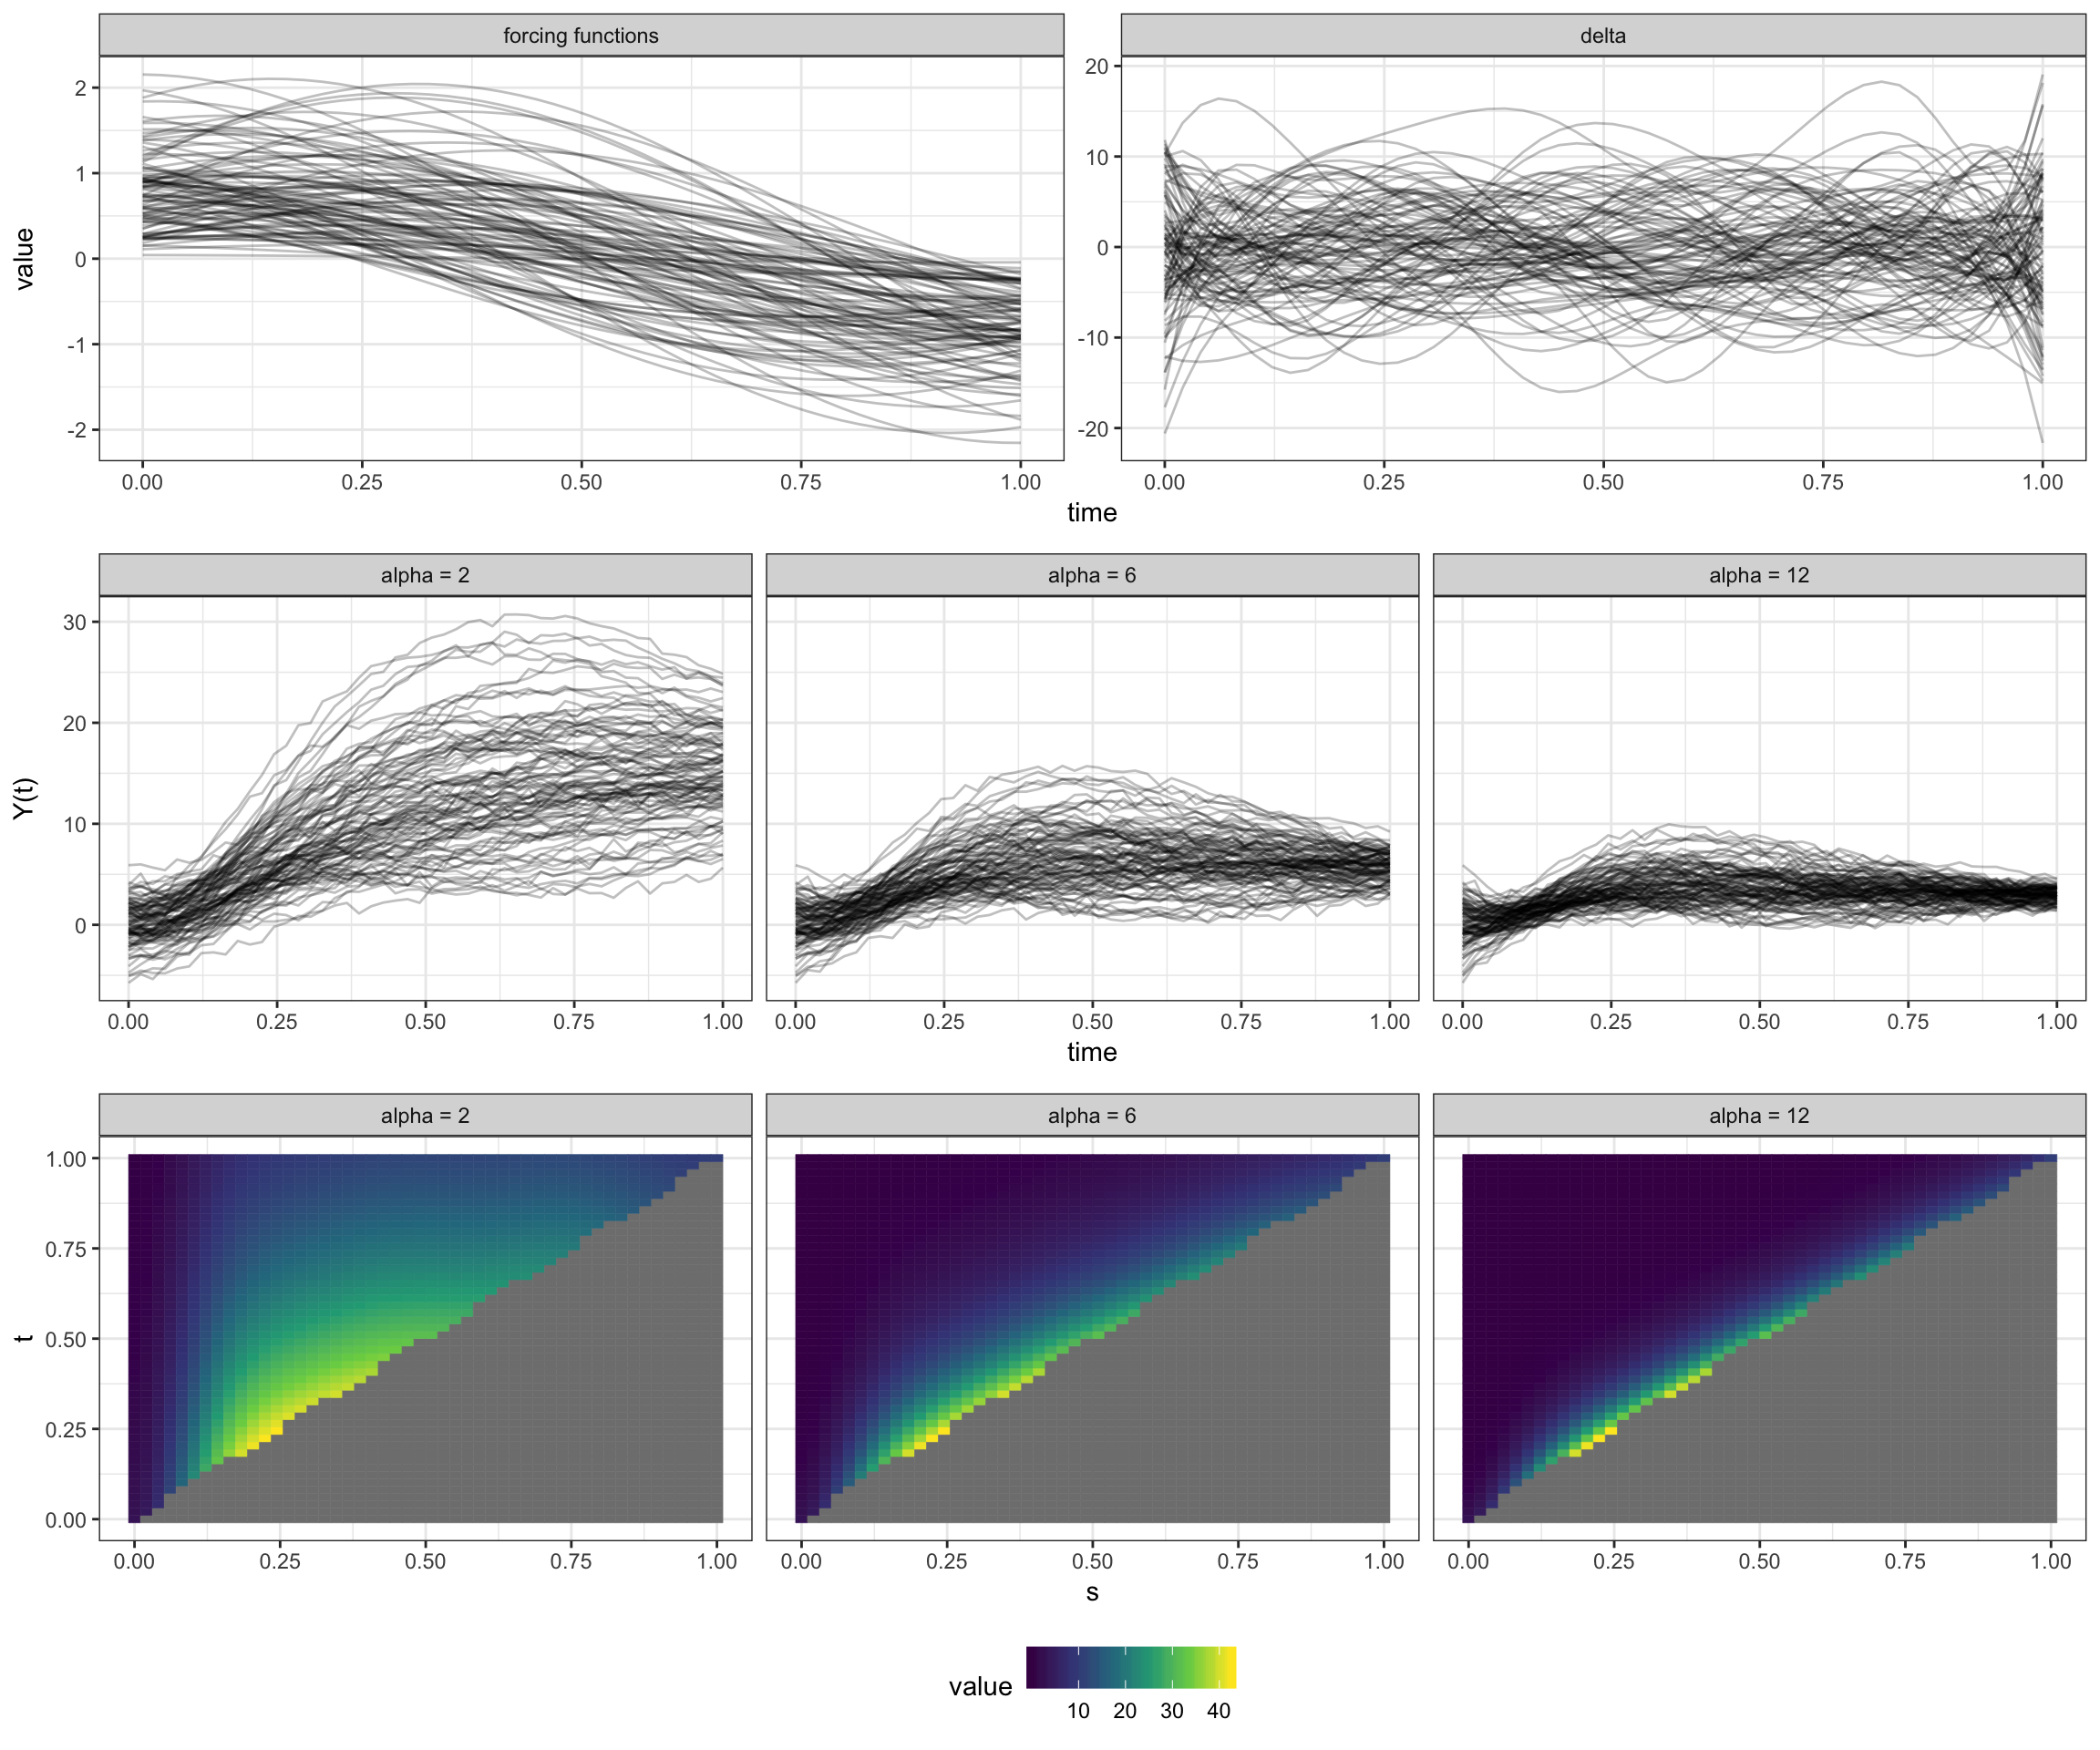
\includegraphics[width=\reprintcolumnwidth]{figs/fig_simdata_RE-1} \caption{This figure shows simulated data when alpha = 2, alpha = 6, and alpha = 12. Top row: Left column shows forcing functions, right column shows shows random effects on the paw velocity scale. Middle row: Observed paw positions for three different values of alpha. When alpha is small initial position has a larger effect on the overall trajectory.  Bottom row: Coefficient surfaces for three different values of alpha.  ADD EQUATIONS TO CAPTION.}\label{fig:sim_data}
\end{figure}

\hypertarget{simulation-design}{%
\subsection{Simulation design}\label{simulation-design}}

Each simulated dataset has \(N = 100\) univariate paw trajectories
\(Y_i(\mathbf{t}))\) with a population intercept \(\mathcal{B}_0(t)\)
and one forcing function \(\mathbf{x}_1(t)\). All trials share the same
equally-spaced grid, \(\mathbf{t}) \in [0, 1]\), of length \(D = 50\).
To reflect how initial values vary across trials in the motivating data,
for each trial \(i\), initial position \(y_i(0)\) is sampled from
\(N(0, 5)\). The forcing function takes the form
\(\mathbf{x}_{i1}(\mathbf{t})) = scale_i \times \sin(\pi_i \mathbf{t}) + shift_i)\),
where \(scale_i\) and \(shift_i\) are randomly-drawn, trial-specific
scale and shift parameters. Random intercepts \(\delta_i(\mathbf{t}))\)
are constructed using 10 B-spline basis functions
\(\mathbf{\Theta}(\mathbf{t}))\) and spline coefficients
\(\mathbf{d}_i\), are drawn from
\(\mathbf{d}_i \sim N(0, \lambda I_{10})\), where \(\lambda = 50\).
Measurement errors \(\epsilon_i(\mathbf{t}))\) are drawn from
\(\epsilon_i(\mathbf{t})) \sim N(0, \sigma^2 I_{D})\), where
\(\sigma^2 = 0.1\), an amount of residual variance which is comparable
to that seen in our motivating data.

Figure \ref{fig:sim_data} shows three simulated datasets when
\(\alpha = 2\), \(\alpha = 6\), and \(\alpha = 12\). The middle and
bottom rows show paw position trajectories \(Y_i(t)\) and coefficient
surfaces \(e^{-\alpha (t-s)} \mathcal{B}_1(s)\), respectively, across
\(\alpha\) values. The top row shows (from left to right) forcing
functions \(x_{i1}(t)\) and random intercepts on the derivative scale
\(\delta_i(t)\), which do not depend on \(\alpha\) and are shared across
these three datasets. The middle panel highlights the buffering effect
of \(\alpha\). When \(\alpha = 2\) buffering is high, meaning initial
position has a consistent effect on the overall trajectory over the time
span of the trial. When \(\alpha = 12\) buffering is low, and the impact
of initial position and forcing functions becomes instantaneous.

We evaluate performance of our model as a function of the buffering
parameter \(\alpha\). For each \(\alpha \in (2, 4, 6, 8, 10, 12)\), we
simulate 25 different datasets, and apply the methods described in
Section \ref{sec:methods} to each dataset. For model estimation we
choose \(K_t = 10\) B-spline basis functions. We initialize \(\alpha\)
using a rough grid search over \(\alpha \in [1, 14]\) to find the value
of \(\alpha\) that minimize sum of squared error when
\(\delta_i(t) = 0\). The true initial position \(y_i(0)\) is initialized
using the observed initial position \(Y_i(0)\), and random effects
\(\delta_i(\mathbf{t}))\) are initialized at 0.

\hypertarget{comparison-with-historical-functional-regression}{%
\subsection{Comparison with historical functional
regression}\label{comparison-with-historical-functional-regression}}

We compare \emph{flode} to the historical functional regression model in
(\ref{eq:fhist_mod}). This model is implemented using the \texttt{pffr}
function from the \texttt{refund} package in \texttt{R} \citep{refund},
and is denoted \emph{fhist} in text and figures below. Comparisons
between \emph{flode} and \emph{fhist} are made based on recovery of the
true coefficient surfaces. We define the surface from the \emph{flode}
model as \(\beta_1^{flode}(s, t) = e^{-\alpha (t-s)} \mathcal{B}_1(s)\),
and compare it to \emph{fhist} surface \(\beta_1^{fhist}(s, t)\).
Surface recovery accuracy is quantified using the integrated squared
error (ISE), where for \emph{flode}
\(ISE = \int_t \int_s \left\{ \beta_1(s, t) - \widehat{\beta}_1^{flode}(s, t) \right\}^2 ds dt\)
and for \emph{fhist}
\(ISE = \int_t \int_s \left\{ \beta_1(s, t) - \widehat{\beta}_1^{fhist}(s, t) \right\}^2 ds dt\).
We also compare \emph{flode} and \emph{fhist} based on recovery of the
true measurement error, \(\sigma^2 = 0.1\).

The buffering parameter \(\alpha\) is an important component of the
\emph{flode} model but is not estimated by the historical functional
model. In figures below, in addition to comparing the performance of
\emph{flode} and \emph{fhist}, we also visualize how well our
\emph{flode} implementation recovers the true value of \(\alpha\) across
simulation scenarios.

\hypertarget{simulation-results}{%
\subsection{Simulation results}\label{simulation-results}}

Figure \ref{fig:sim_results} shows results from a single simulated
dataset with \(\alpha = 6\) and 100 trials. From top to bottom, rows
show observed (gray) and fitted (red) values, true (gray) and estimated
(red) random effects on the data scale, and coefficient surfaces. The
top and middle rows show results for \emph{fhist} (left column) and
\emph{flode} (right column), while the bottom row shows the
\emph{fhist}, \emph{flode}, and true surfaces, respectively. For this
simulated dataset, both \emph{flode} and \emph{fhist} produce reasonable
results for the fitted values. However, it is clear from the random
effects and coefficient surfaces that \emph{flode} and \emph{fhist} are
estimating these overall fits in different ways, and that \emph{flode}
is recovering the true surface values.

Figure \ref{fig:sim_surfaceErr} summarizes results for \emph{flode} and
\emph{fhist} across datasets generated using different values of
\(\alpha\). The left panel shows \(\log ISE\), and the right panel shows
estimated measurement errors \(\widehat{\sigma}^2_{flode}\) and
\(\widehat{\sigma}^2_{fhist}\). Across values of \(\alpha\),
\emph{flode} outperforms \emph{fhist} in terms of the \(ISE\), which is
consistent with observations in Figure \ref{fig:sim_results}. At low
values of \(\alpha\), the difference in performance between the methods
is smaller, and \(ISE\) variability for \emph{flode} is high when
\(\alpha = 2\). Measurement error is slightly biased away from the true
value \(\sigma^2 = 0.1\) for both models, though the bias is larger for
the \emph{fhist} model across values of \(\alpha\). The \emph{flode}
model is slightly overfitting the data, while \emph{fhist} underfits the
data.

Figure \ref{fig:sim_alpha} shows estimated values \(\widehat{\alpha}\)
(top row) and random effects variance \(\widehat{\lambda}\) (bottom row)
from \emph{flode} across datasets with different true values of
\(\alpha\). Our \emph{flode} implementation recovers close to the true
value of \(\alpha\), though values are slightly biased towards zero for
datasets with higher true values of \(\alpha\). Our estimates for
\(\lambda\) are also slightly biased towards zero, an effect which is
also pronounced for higher true values of \(\alpha\). Though not shown,
the simulations described above were also performed at the increased
sample size of \(N = 200\) trials. When sample size increases, the
variance of \(\alpha\) and \(\lambda\) estimates decreases, the
algorithm converges in fewer iterations, and \(ISE\) values are lower.

\begin{figure}
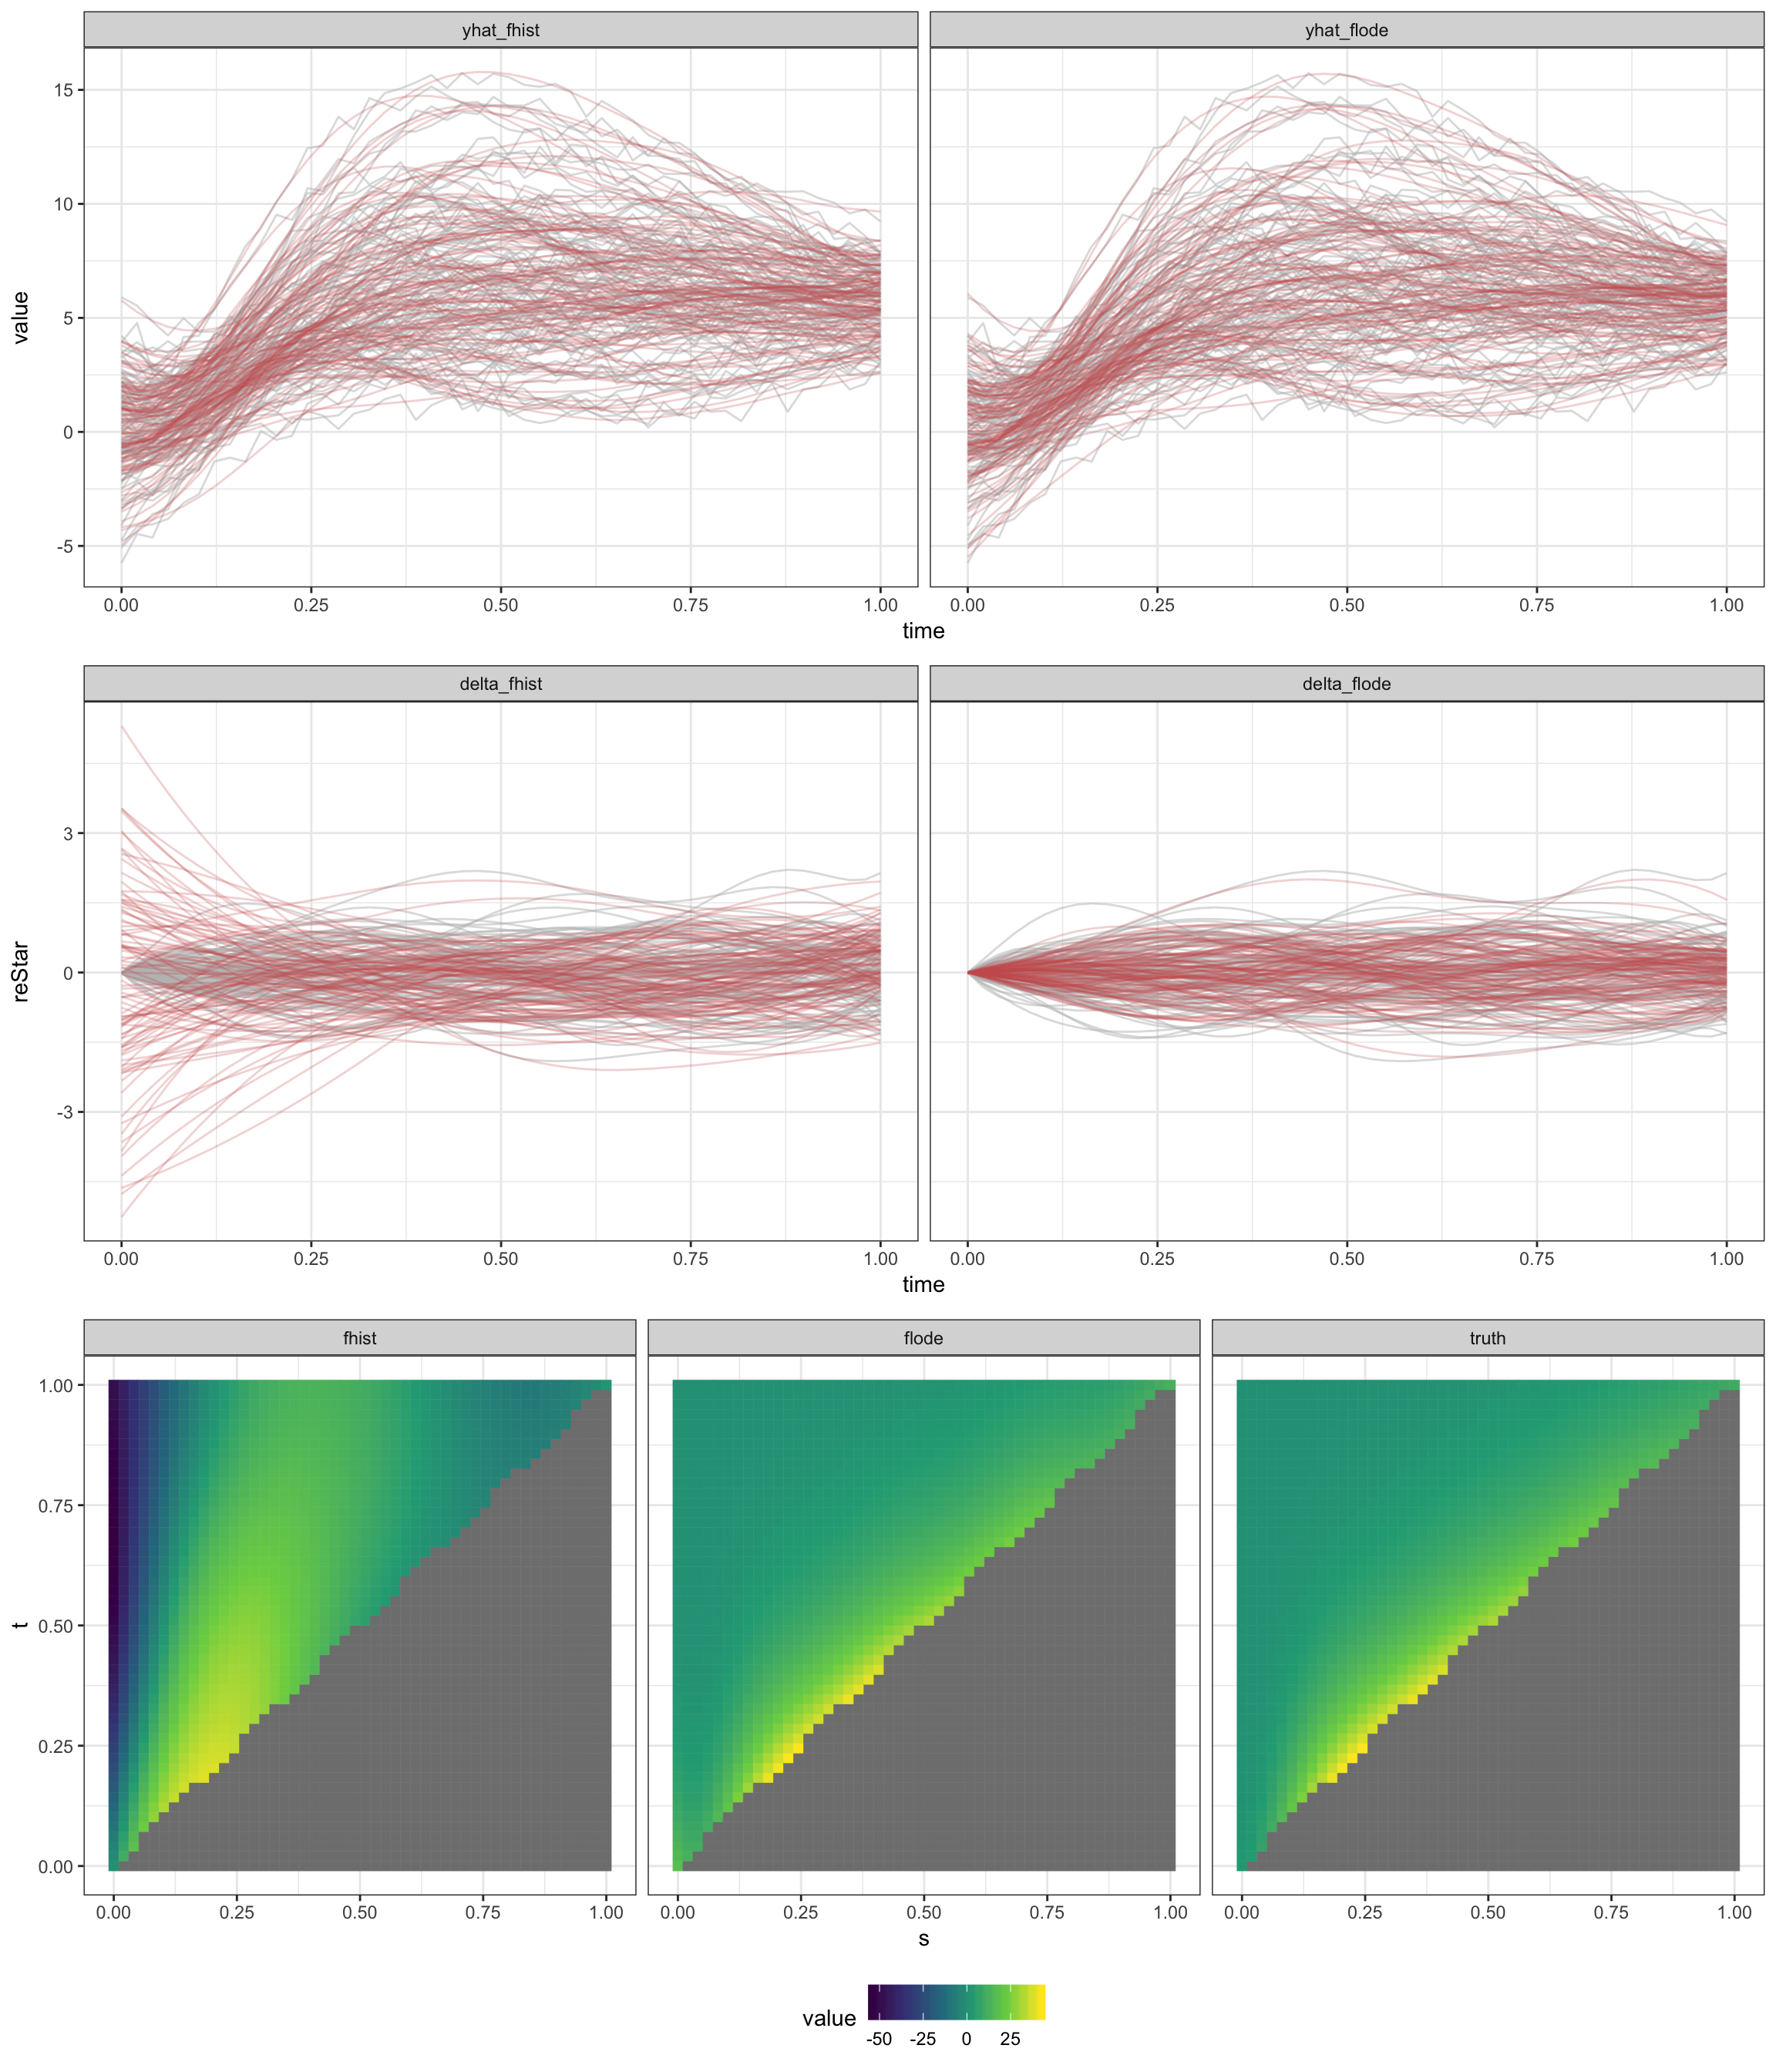
\includegraphics[width=\reprintcolumnwidth]{figs/fig_sim_results-1} \caption{Top row: Fitted values from *fhist* and *flode*. Second row: Residuals from *fhist* and *flode*.  Third row: Random intercepts from *fhist* and *flode*. Values for *flode* are shown on the data scale so that they are comparable with *fhist*. Bottom row: Estimated surfaces from *fhist* and *flode*. Both models were run on the same dataset with ADD EQUATIONS}\label{fig:sim_results}
\end{figure}

\begin{figure}
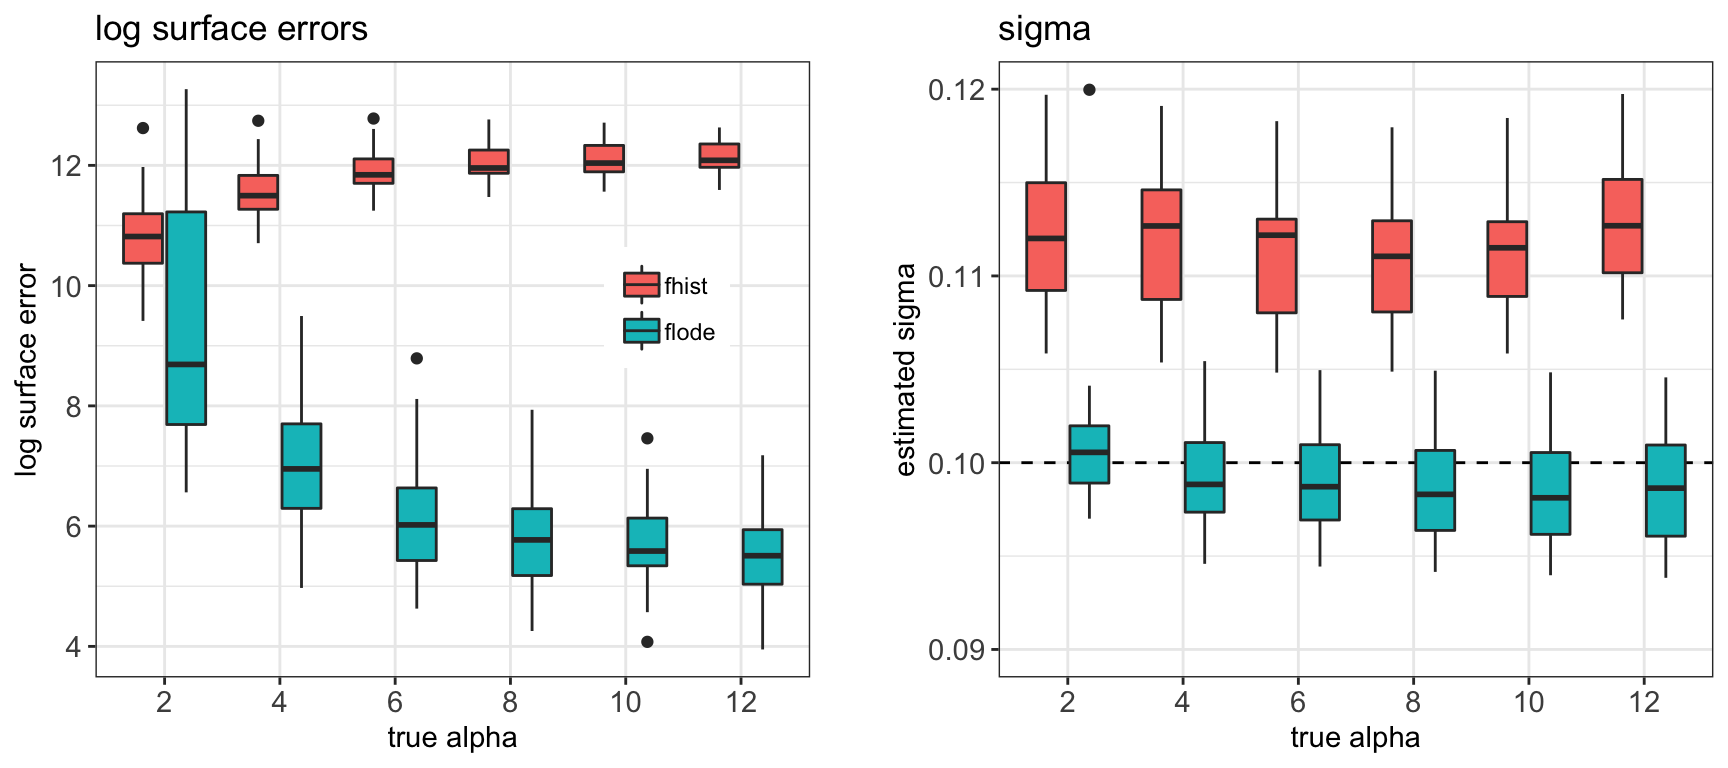
\includegraphics[width=\reprintcolumnwidth]{figs/fig_sim_surfaceErr-1} \caption{Log surface errors}\label{fig:sim_surfaceErr}
\end{figure}

\begin{figure}
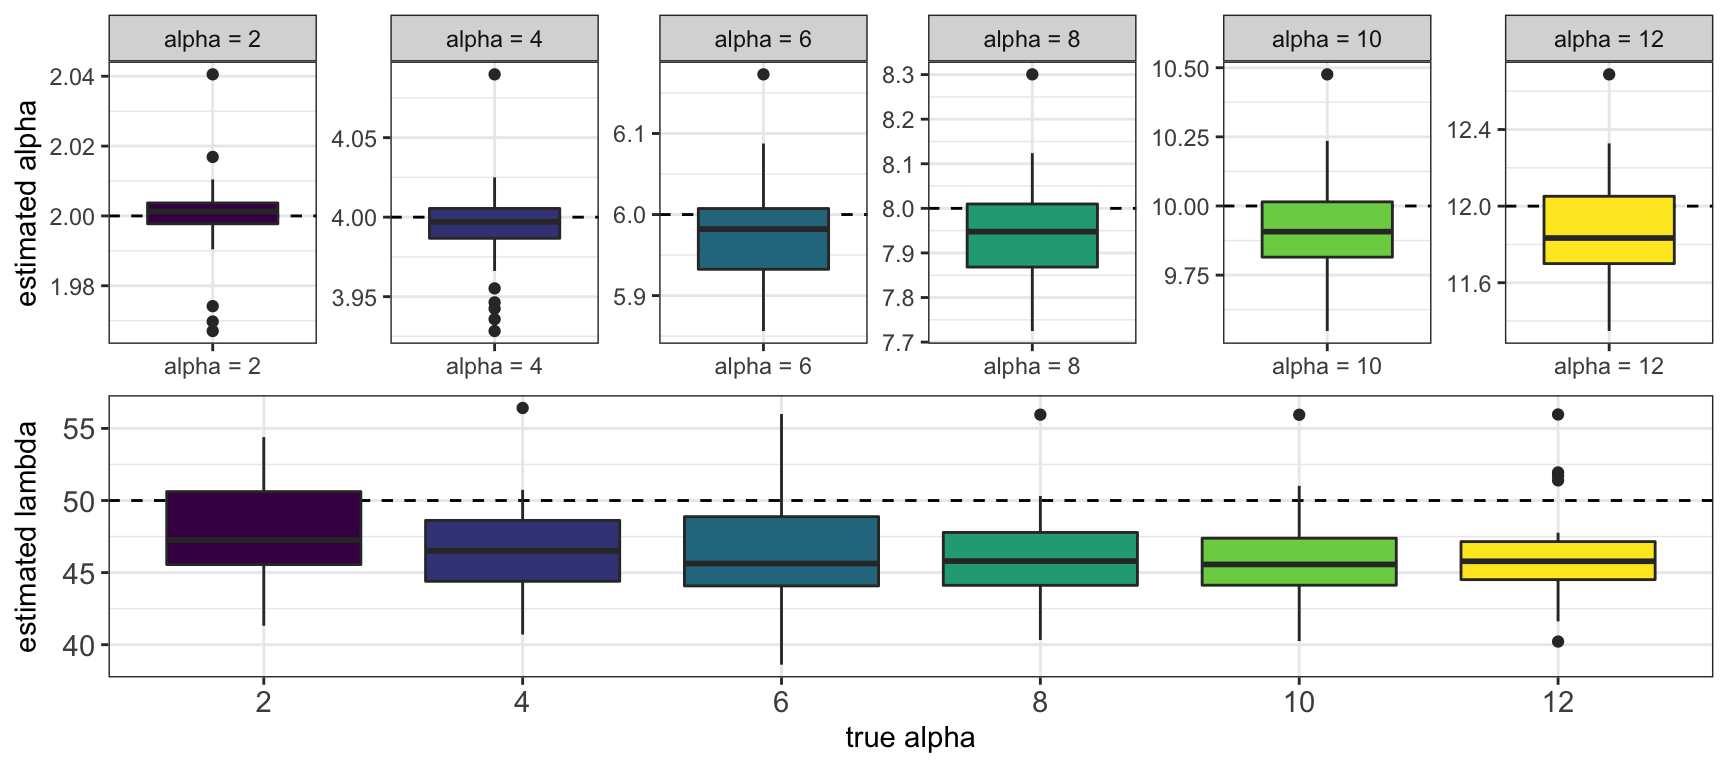
\includegraphics[width=\reprintcolumnwidth]{figs/fig_sim_alpha-1} \caption{alpha simulations}\label{fig:sim_alpha}
\end{figure}

\hypertarget{data-analysis}{%
\section{Data Analysis}\label{data-analysis}}

\label{sec:results}

In this section, we apply the methods described in Section
\ref{sec:methods} to the mouse paw trajectory data introduced in Section
\ref{sec:data}. Our dataset consists of 147 paw trajectory trials from a
single mouse, where each trajectory was collected under the same
experimental conditions. Accompanying paw trajectories are measurements
of brain activity in the motor cortex, as summarized by GPFA
\citep{yu2009}, for a total of 5 forcing functions. Position and neural
activity were recorded concurrently at a rate of 500 measurements per
second. We restrict our analysis to the period just before lift (when
the paw leaves a resting location) to just after grasp (when the paw
grasps a food pellet). Because grasp occurred at different times across
trials, we linearly interpolate the data to an even grid of length
\(D = 50\) that is shared across trials.

\begin{figure}
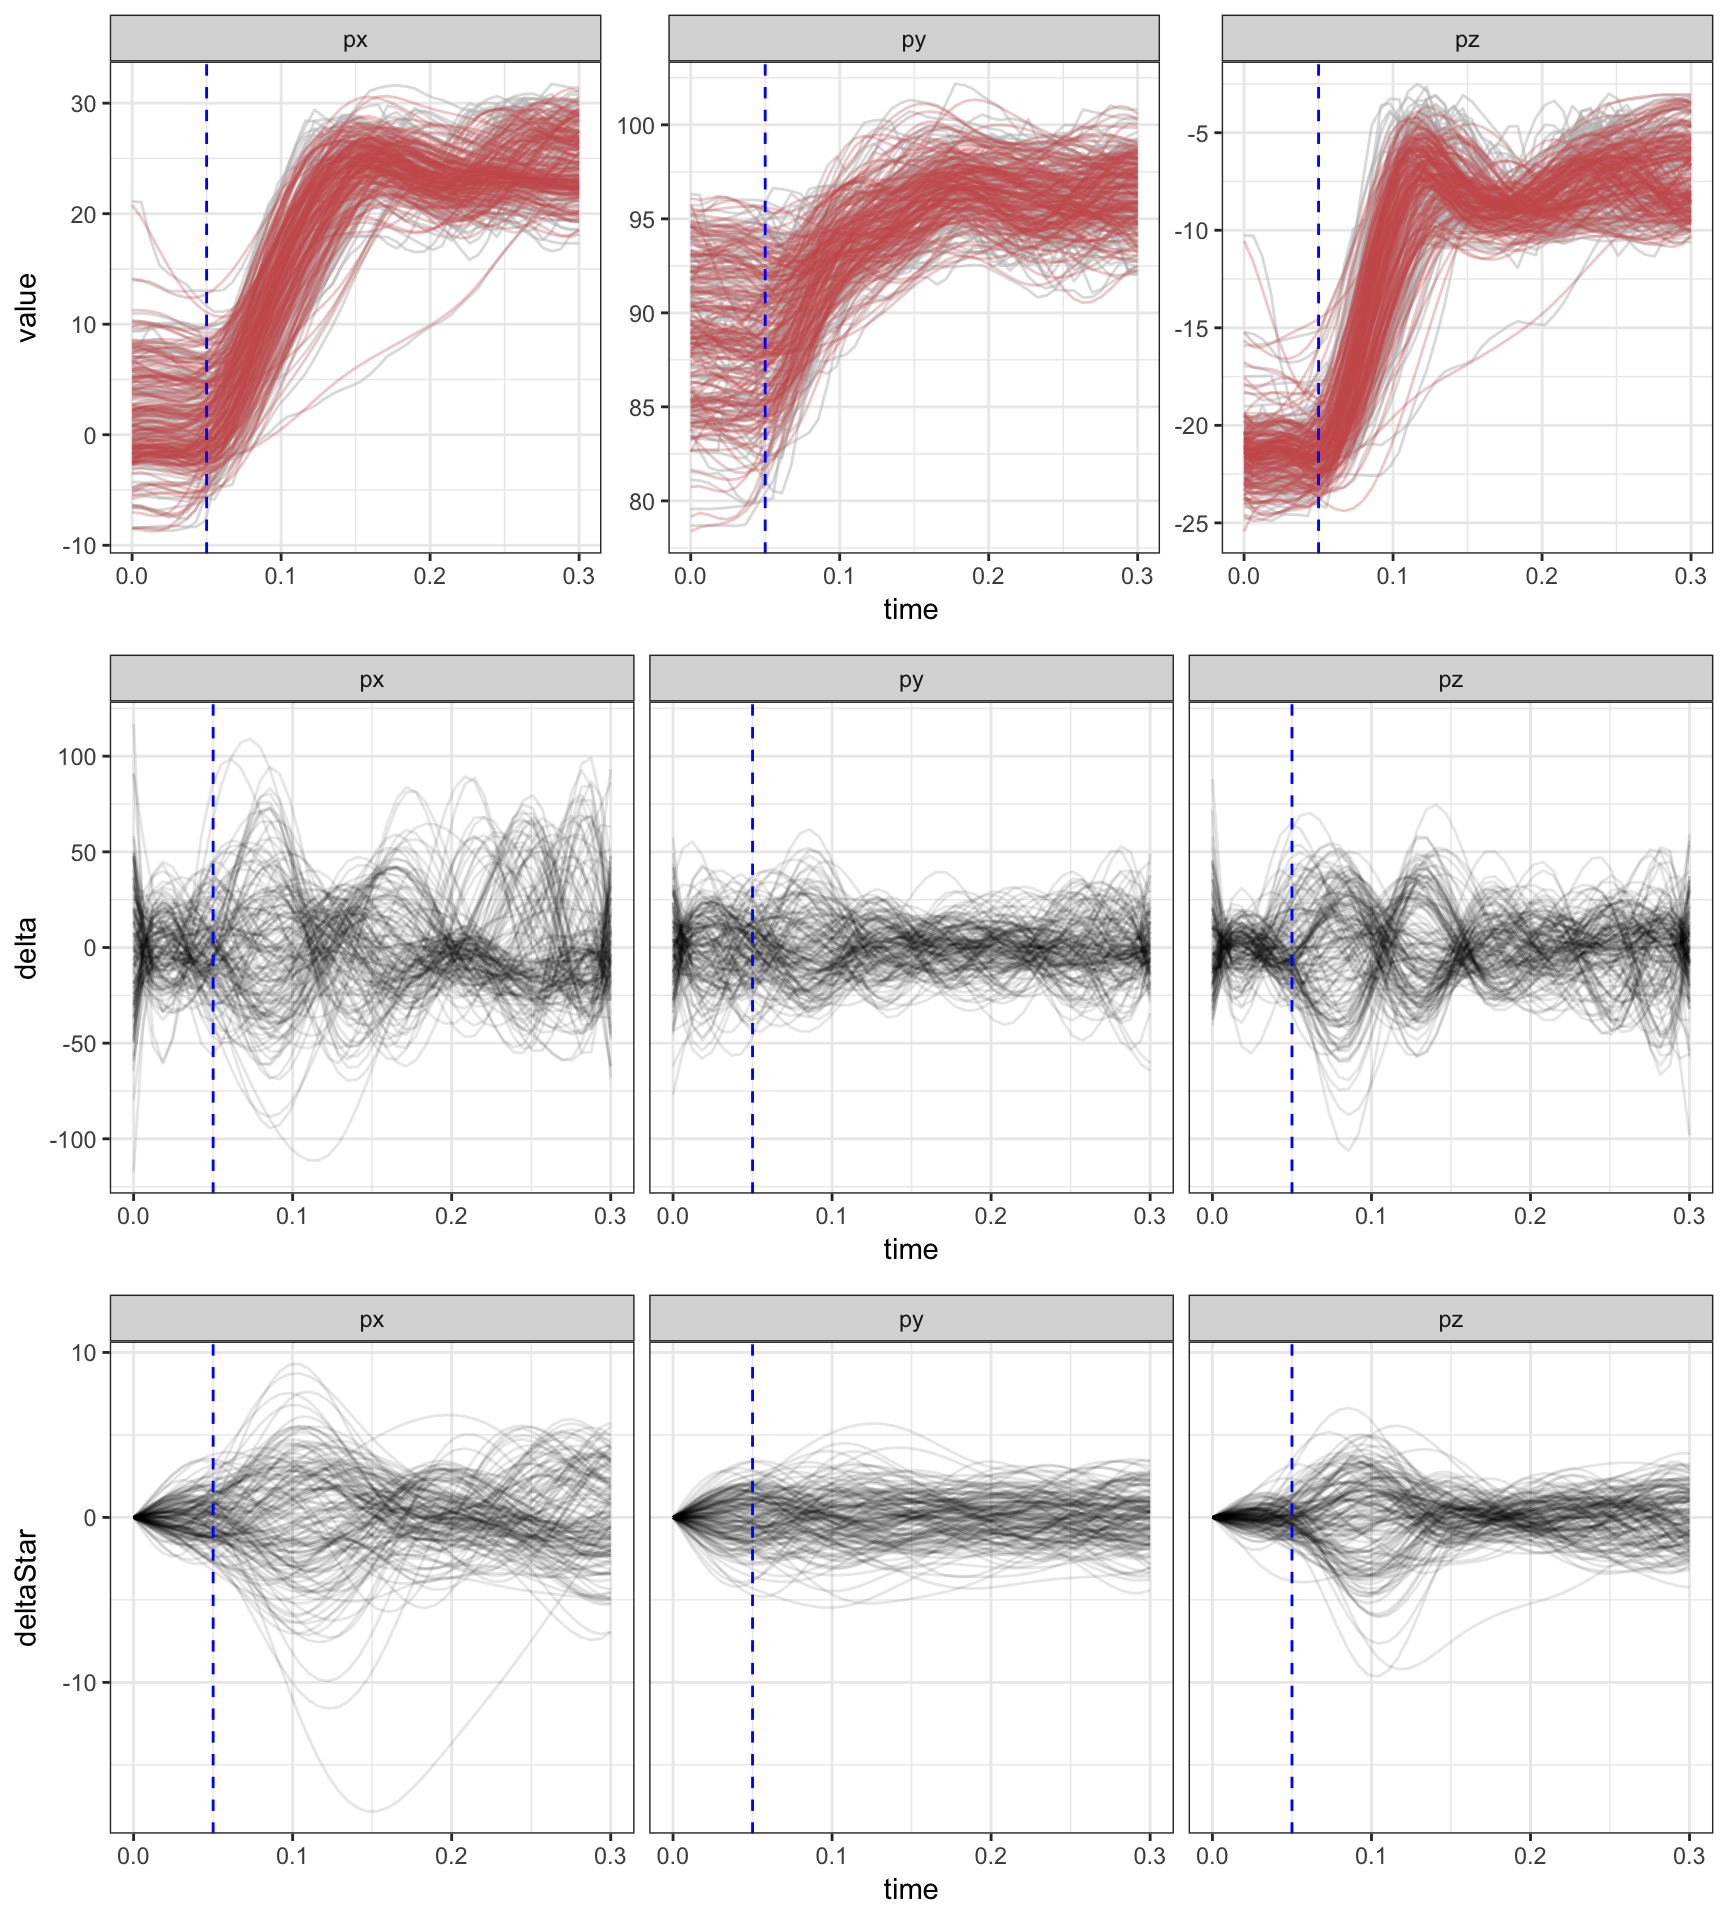
\includegraphics[width=\reprintcolumnwidth]{figs/fig_data_fits-1} \caption{This figure shows fitted values, estimated random effects, and integrated random effects across axes for the paw data. The vertical dotted line occurs at the time of lift for each trial.}\label{fig:paw_fits}
\end{figure}

\begin{figure}
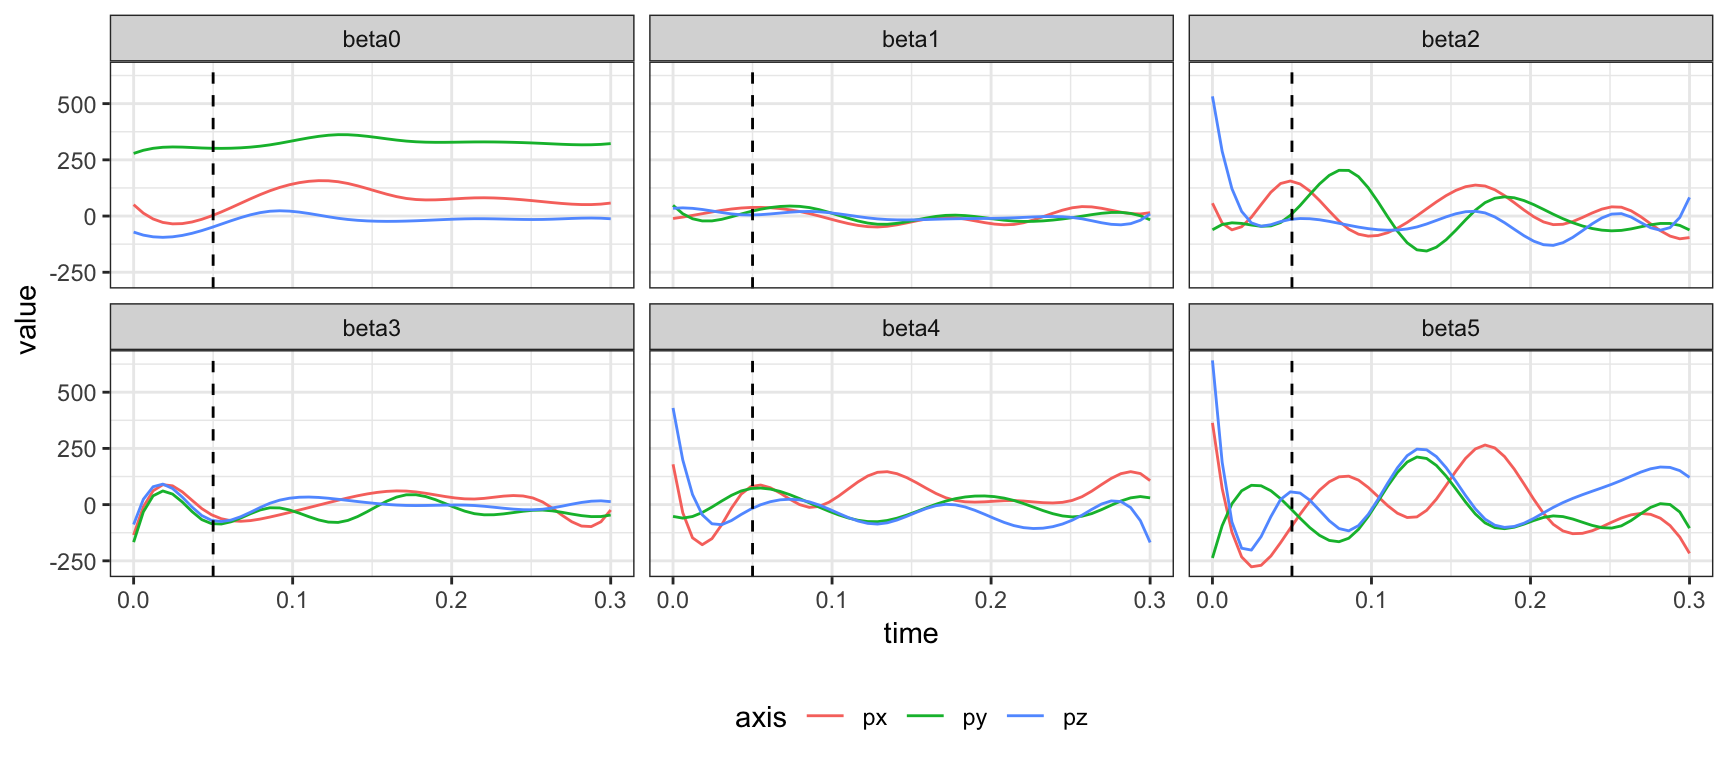
\includegraphics[width=\reprintcolumnwidth]{figs/fig_data_beta-1} \caption{This figure shows fitted intercept and coefficient functions across axes for the paw data. The vertical dotted black line occurs at the point of lift.}\label{fig:paw_betas}
\end{figure}

\begin{figure}
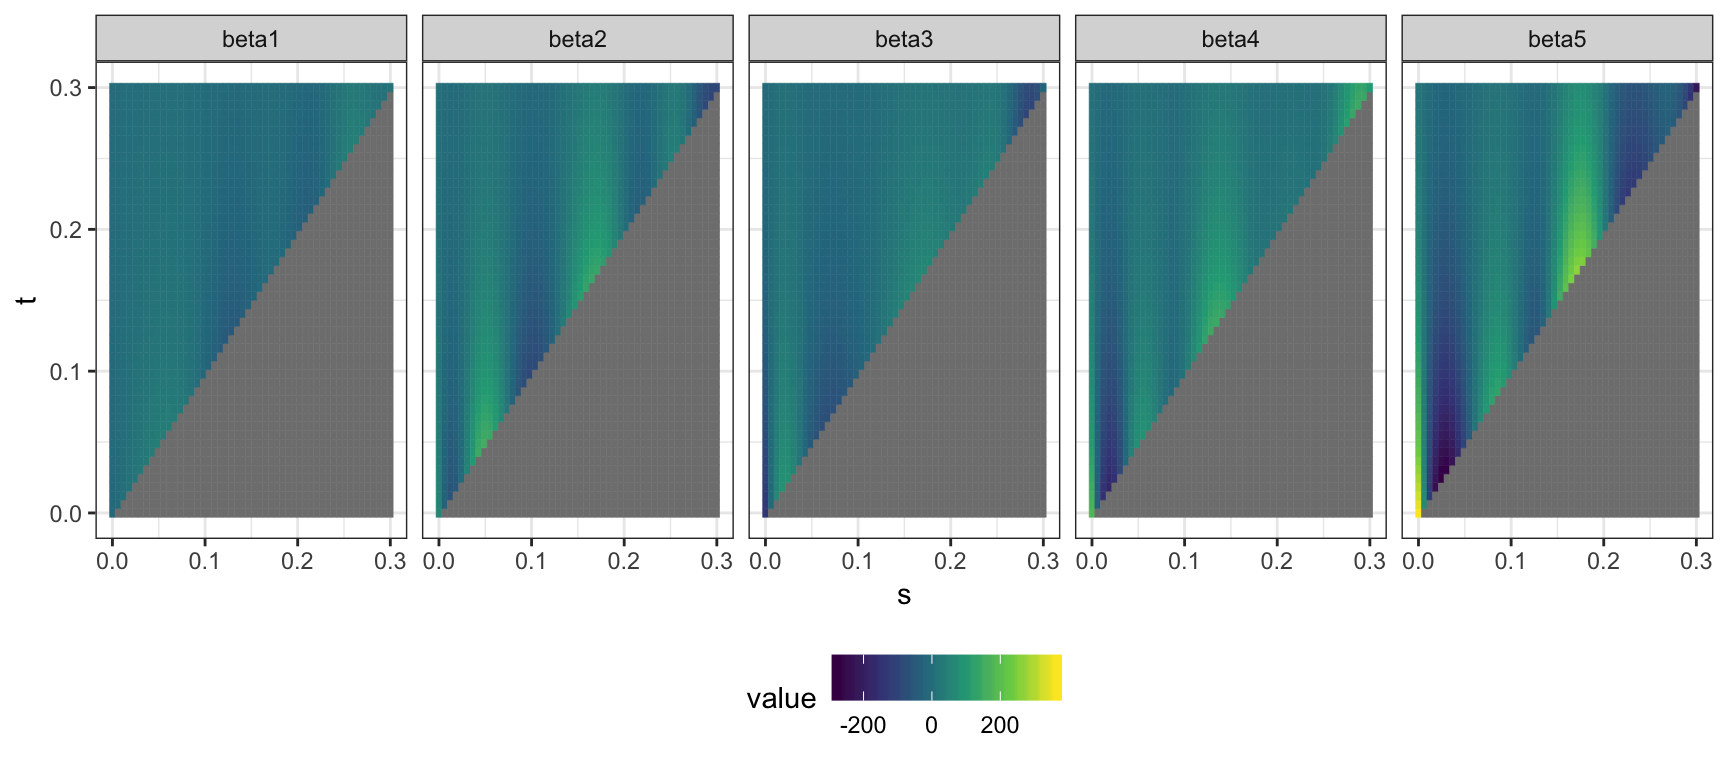
\includegraphics[width=\reprintcolumnwidth]{figs/fig_data_surfaces-1} \caption{This figure shows estimated surfaces}\label{fig:paw_surfaces}
\end{figure}

We present a univariate analysis of the trajectories in the \(x\),
\(y\), and \(z\) directions. For each axis, we set the number of
B-spline bases to \(K_t = 10\) and fit the \emph{flode} model in
(\ref{eq:flode_mod}). The parameter \(\alpha\) was initialized by doing
a grid search over values in \([2, 12]\) to find the value,
\(\alpha_0\), that minimizes the model when each \(\delta_i(t) = 0\).
This \(\alpha_0\) was then used as a starting value for the \emph{flode}
algorithm. The results of this analysis are described and interpreted
below.

Estimated values of the buffering parameter, are, for each axis,
\(\widehat{\alpha}_x = 3.01\), \(\widehat{\alpha}_y = 3.50\), and
\(\widehat{\alpha}_z = 3.01\). These values are close, indicating
similar amounts of buffering across axes. For Figure \ref{fig:paw_fits},
the first row shows observed (gray) and fitted (red) values for paw
position. The second row shows random effects on the derivative scale
for each trial, \(\delta_i(t)\). The third row shows these random
effects on the data scale, \(\int_s e^{-\alpha (t-s)}\delta_i(s)ds\).
The first, second, and third columns show results for the \(x\), \(y\),
and \(z\) axis, respectively. The dotted line through each plot occurs
at \(t= 0.05\) seconds, which is the time of paw lift for each trial.
The fitted values are capturing the data well. The random effects show
more residual variance right after lift (during the time of the actual
reach) than in other parts of the trial, suggesting that maybe there is
something driving the reaching movement that we are not measuring.

Coefficient functions and coefficient surfaces are shown in Figures
\ref{fig:paw_betas} and \ref{fig:paw_surfaces}, respectively. For
surfaces we only show results from the \(x\) axis; results from the
\(y\) and \(z\) axes followed the same trends.

\hypertarget{discussion}{%
\section{Discussion}\label{discussion}}

\label{sec:discussion}

We present \emph{flode}, a nonlinear regression model that has context
in both functional data analysis and systems of ordinary differential
equations. Drawing from both of these literatures is necessitated by our
application; the differential equations formulation of our model allows
for an interpretation of our paw data as trajectories whose speed and
position are dynamically influenced by inputs from the brain, and tools
from functional data analysis allow us to efficiently model repeated
observations that are trajectories while incorporating smoothness in the
coefficient functions. Though we are motivated by a specific application
in neurobiology, our methods are general and broadly useful for anyone
trying to study a dynamical system of inputs and outputs where the
outputs are functions over time. Our novel method compares favorably
with historical functional regression in the simulation settings we
examined, and produces reasonable results for our motivating data. Our
methods are publicly available in an \texttt{R} package.

We believe this work is an exciting addition to a nascent field in
statistics, with many possible future directions. A study on the
asymptotics of the coefficients estimated in this model so that large
sample confidence intervals and hypothesis tests can be computed would
help researchers draw inferences about the relationships between inputs
and outputs of the dynamical system. Extensions to include more complex
systems of ordinary differential equations, including higher order and
non-linear ODEs would increase the flexibility of our modeling framework
and allow for the study of a larger class of repeated measurements of
dynamical systems.

The \emph{flode} model was developed based on our current understanding
of biological processes, and we're working to expand that framework to
include more complex inputs. For example, we view the \(\delta_i(t)\)
term as capturing correlation due to unmeasured forces acting on the
system. Prior work suggests that this signal is coming from the thalamus
and it would be useful to work with neurobiologists to collect data and
develop a model that incorporates neural information from multiple
sources within the brain, with the ultimate goal of recreating reaching
movements based only on initial position and neural activity patterns.

\hypertarget{repro-items}{%
\section{Repro items}\label{repro-items}}

Add reproducibility checklist below

% -------------------------------------------------------------------------------------------------------------------
%   Appendix  (optional)

%\appendix
%\section{Appendix title}

%If only one appendix, please use
%\appendix*
%\section{Appendix title}


%=======================================================

%Use \bibliography{<name of your .bib file>}+
%to make your bibliography with BibTeX.

%=======================================================

\bibliography{biblio.bib}


\end{document}
